The purpose of this chapter is to benchmark and evaluate Memcached performance. Firstly, we will focus on Memcached performance ``out of the box''. Secondly, we will examine Memcached scalability in respect to threads which will provide us with an optimization baseline. It is worth noting that majority of Memcached user will end up using the default configuration, perhaps with increased threading level. Subsequently, we will explore the impact of assigning individual threads to CPU cores as well as the impact interrupt processing has on Memcached. Furthermore, we will explore a multi-instance setup as well as the impact object size has on Memcached performance. Finally, we will turn our attention to the distribution of cache keys.

Throughout this chapter, we will focus primarily on latency, 99th percentile latency and throughput. Where relevant, we will explore additional attributes. Unless otherwise stated, all performance tuning is done to meet a Quality of Service (QoS) constraint of 99th percentile latency under 1 millisecond.

\section{Shiny Fresh Memcached}
Firstly, let us focus on Memcached performance ``out of the box'', that is, Memcached with a default configuration. When we tear down the wrapping paper of a Memcached distribution, we are presented with two important configuration options - a) The port number memcached will listen on and b) the amount of memory we allocate to Memcached which determines the total capacity of the cache. For the purposes of this paper, we use port number 11120. The amount of memory we allocate to memcached is dependent on the total amount of memory available on the host machine as well as any additional workload on the host. In our case, we are the sole workload with a total of 8GB memory available to us. Throughout this paper, we choose to allocate 6 GB of memory to Memcached, leaving 2 GB for the operating system or remaining unused. Table \ref{tab:m_default_config} outlines the configuration options including relevant defaults. It is worth noting that in the default configuration Memcached runs with 4 threads.

\begin{table}[h!]
\centering
\begin{tabular}{| c c c |}
 \hline
 Configuration Option & Explanation & Value\\ [0.5ex]
 \hline\hline

 -d & Run in Daemon Mode & true \\
 -p & Port number & 11120 \\
 -t & Number of Threads & 4 (default) \\
 -m & Memory Allocated & 6144 (6GB) \\

 \hline

\end{tabular}
\caption{Memcached Configuration Options.}
\label{tab:m_default_config}
\end{table}

Given the configuration outlined in Table \ref{tab:m_default_config}, we can proceed and launch Memcached on the server with the following command:
\begin{lstlisting}
memcached -d -p 11120 -m 6144
\end{lstlisting}


Secondly, we configure the clients responsible for generating cache workload. In order to determine a saturation point of the serve cache, we increase the workload exerted by the clients linearly. Initially, we consider a workload provided by 3 threads and 1 connection per each workload generating server. Subsequently, the number of connections is increased linearly until a saturation point is found or QoS requirements are no longer satisfied. For the benchmark, and indeed for the rest of the paper unless otherwise stated, we consider an object size of 64 bytes. With object sizes of 64 bytes, we aim to generate a sufficiently large dataset in order to exceed the memory capacity provisioned for Memcached. In this case, we define the key space to be between 1 and 100 million, yielding a dataset 6.4GB large. Table \ref{tab:m_memtier_default} outlines the configuration options used.

\begin{table}[h!]
\centering
\begin{tabular}{| c c c |}
 \hline
 Configuration Option & Explanation & Value\\ [0.5ex]
 \hline\hline

 -s & Server & nsl200 (server hostname) \\
 -p & Port number & 11120 \\
 -c & Number of Connections & [1..10] \\
 -t & Number of Threads & 3 \\
 --key-minimum & Smallest key & 1 \\
 --key-maximum & Largest key & 100 000 000 \\
 --random-data & Generate Random Data & true \\
 --data-size & The size of data in bytes & 64 \\

 \hline

\end{tabular}
\caption{Memtier Configuration Options}
\label{tab:m_memtier_default}
\end{table}

The memtier\_benchmark (Memtier) can be launched with the following command:
\begin{lstlisting}
  memtier -s <server> -p 11120 -c <connections> -t 3
    --random-data
    --key-minimum=1
    --key-maximum=100000000
    --random-data
    --data-size=64
\end{lstlisting}

The application start commands are provided for clarity and will be omitted in subsequent benchmarks as they can be directly constructed from the configuration tables.

\subsection{Latency, Throughput and Number of Connections}

Firstly, we are interested in the relationship between throughput, latency and the number of connections. The relationship is shown in Figure \ref{fig:memcached-default-latency-vs-ops}. Latency, both mean and 99th percentile, are plotted on the left vertical axis, the number of operations per second is plotted on the right vertical axis and the number of connections used is on the horizontal axis.

\begin{figure}[h]
    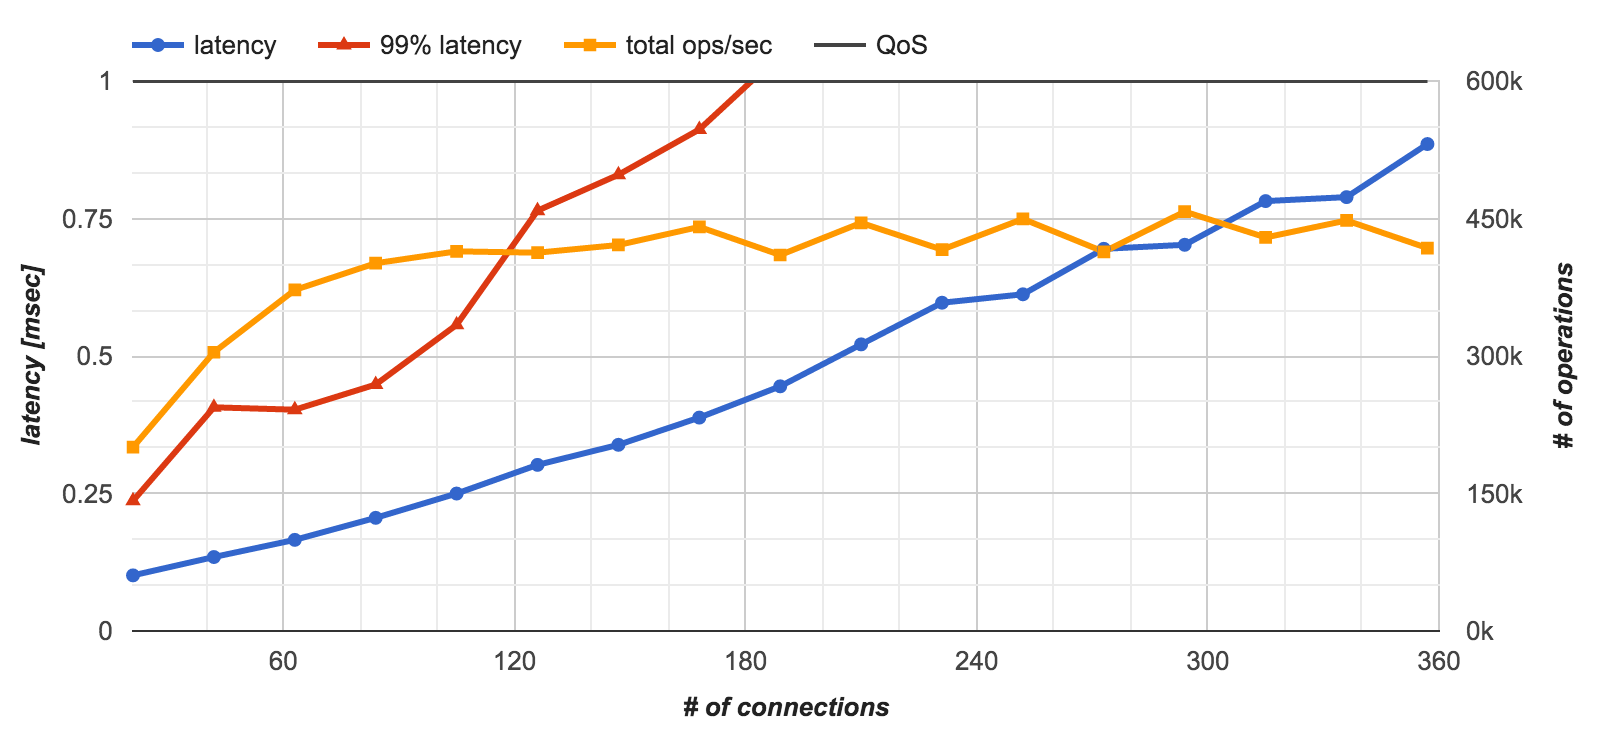
\includegraphics[width=\textwidth]{./res2/m_baseline_latency.png}
    \caption{Latency \& Throughput vs Number of Connections}
    \label{fig:memcached-default-latency-vs-ops}
\end{figure}

As the number of connection increases, so does mean latency. There is a linear relationship between the mean latency and the number of connections. This is an expected result, as the load increases linearly, we expect the mean latency to increase linearly too. An increase in the number of connections by 21 results in increased mean latency by approximately 0.09ms.

The 99th percentile latency increases linearly with the number of connections until we reach 105 connections. A further increase in the number of connections results in a disproportionately greater increase in tail latency. The maximum number of connections satisfying the QoS occurs at 147 connections and tail latency at 0.99ms. A further increase in load results in a steeper increase in tail latency. We can observe as the load increases, the tail latency diverges from the mean latency and increases at a faster pace.

The number of operations per second increases linearly with the number of connections and reaches a peak of 238k requests per second at 147 connections (within QoS). The total throughput appears to be largely unaffected by the steep increase in tail latency in this benchmark.


\subsection{CPU Utilization}

Secondly, we consider the effect of the workload on the Memcached server in terms of CPU Utilization. The CPU utilization is monitored through the \textit{mpstat} \cite{mpstat} utility which reports the percentage of CPU utilization broken down into multiple categories. The following table \cite{mpstat} summarizes the responsibilities of each category.

\begin{enumerate}
    \item [\%usr] Show the percentage of CPU utilization that occurred while executing at the user level (application).
    \item [\%sys] Show the percentage of CPU utilization that occurred while executing at the system level (kernel). Note that this does not include time spent servicing hardware and software interrupts.
    \item [\%iowait] Show the percentage of time that the CPU or CPUs were idle during which the system had an outstanding disk I/O request.
    \item [\%irq] Show the percentage of time spent by the CPU or CPUs to service hardware interrupts.
    \item [\%soft] Show the percentage of time spent by the CPU or CPUs to service software interrupts.
    \item [\%idle] Show the percentage of time that the CPU or CPUs were idle and the system did not have an outstanding disk I/O request.
\end{enumerate}

For the context of this paper, \textit{\%usr} corresponds directly to the CPU utilization used by Memcached as it is the only application running on the server.

Furthermore, \textit{\%soft} represents the software interrupt issued by \textit{libevent} when a new file descriptor is available for processing, that is, a new request is available to be processed or a response is ready to be handed over to the network stack.

\begin{figure}[h]
    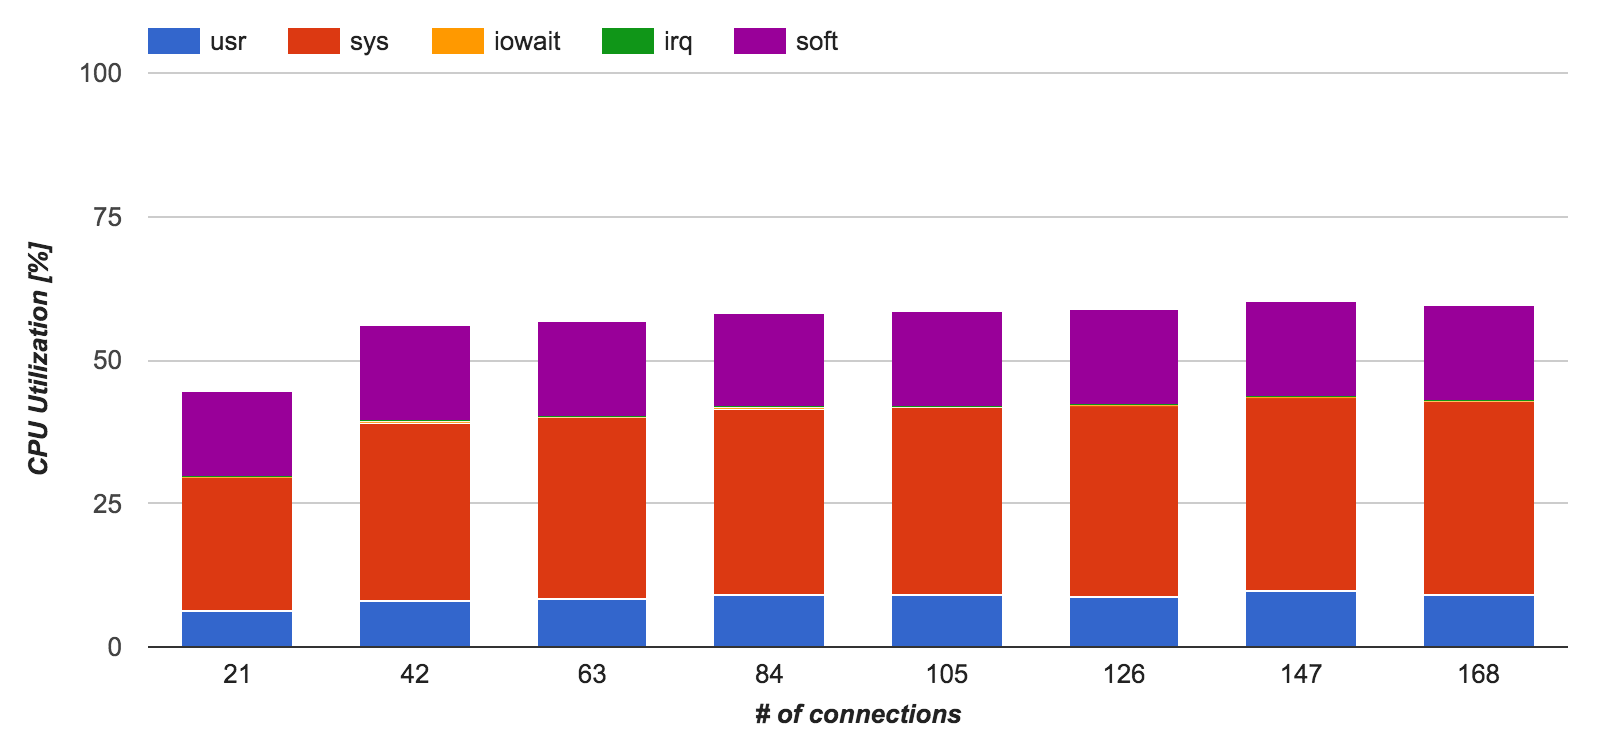
\includegraphics[width=\textwidth]{./res2/m_baseline_cpu.png}
    \caption{CPU Utilization for Out of the Box Configuration of Memcached}
    \label{fig:m_baseline_cpu}
\end{figure}

Figure \ref{fig:m_baseline_cpu} outlines the CPU Utilization broken down into mpstat categories. Note that unallocated percentage constitutes the \textit{idle} percentage of the CPUs.

Memcached utilization (\textit{usr}) increases slightly as the number of connections increases, however, overall remains stable and accounts for at most 9\% of the total utilization. The kernel (\textit{sys}) accounts for 33\%, a significant portion of the CPU utilization relative to other categories. The CPU utilization dedicated to processing software interrupts (\textit{soft}) accounts for 16\% of the total CPU utilization. This makes the second most significant category in the benchmark. Disk IO accounts for 0\% of total utilization as all data is stored in memory and we do not need to access the disk. Hardware interrupts (\textit{irq}) account for 0.01\% of total utilization.

Overall, CPU utilization starts at 48\% and increases to 60\% as the number of connections increases. We can observe that at this CPU utilization we have not been able to fully utilize the server resources. Additionally, the kernel and software interrupts account for majority of the total CPU utilization. This is indicative of a larger pattern of Memcached execution - Memcached performance is dominated by the kernel and network stack. This is consistent with findings in MICA \cite{lim2014mica}.


\subsection{Evaluation}
Given the trends presented in Figures \ref{fig:memcached-default-latency-vs-ops} and \ref{fig:m_baseline_cpu}, we can conclude the ``out of box'' configuration of Memcached does not deliver optimal performance. The number of operations per second could be increased by increasing CPU utilization which in turn  should result in improved tail latency. Additionally, we have been able to observe that the kernel and software interrupt performance dominates the CPU utilization. A simple approach to increasing CPU utilization is to increase the number of threads we provision for Memcached.

% ________________________________________________________

\section{Thread Scalability}
\label{sec:memcached-threads}
In this section, we focus on increasing CPU utilization through the use of multiple threads. We have shown that the default configuration results in underutilization of the server resources and argued that increased CPU utilization should result in improved performance. Memcached, as a high performance object cache, is designed to be executed on a multi-core architecture. Scalability is primarily implemented through the use of multi threading. It is worth noting that multi-threading also results in increased application complexity. Individual threads requiring access to shared data are required to obtain a lock before they can proceed with data manipulation. We design a benchmark which focuses on thread scalability by linearly increasing the number of threads Memcached is provisioned.

Empirically, we expect the best performance to be achieved when there are as many Memcached threads as there are CPU cores. The cache server is equipped with 6 CPU cores and therefore we would expect 6 threads to maximize performance. This is also suggested by Leverich and Kozyrakis \cite{leverich2014reconciling}. Utilizing less threads should result in underutilization of the CPU leading to sub-optimal throughput. More than 6 threads should conversely result in increased context switching overhead and therefore should lead to increased latency.

Utilizing results about the number of connections from previous section, we configure a constant level of workload with 3 Memtier threads and 7 connections per each thread. We maintain the same key-object configuration as in previous benchmark. The configuration details of the Memtier benchmark are outlined in Table \ref{tab:m_threads_memtier}.

\begin{table}[h!]
\centering
\begin{tabular}{| c c c |}
 \hline
 Configuration Option & Explanation & Value\\ [0.5ex]
 \hline\hline

 -s & Server & nsl200 (server hostname) \\
 -p & Port number & 11120 \\
 -c & Number of Connections & 7 \\
 -t & Number of Threads & 3 \\
 --key-minimum & Smallest key & 1 \\
 --key-maximum & Largest key & 100 000 000 \\
 --random-data & Generate Random Data & true \\
 --data-size & The size of data in bytes & 64 \\

 \hline

\end{tabular}
\caption{Memtier Configuration Options}
\label{tab:m_threads_memtier}
\end{table}

Memcached, on the other hand, is configured to increase the number of threads in each consecutive benchmark. Table \ref{tab:m_threads_memcached} outlines the configuration used.

\begin{table}[h!]
\centering
\begin{tabular}{| c c c |}
 \hline
 Configuration Option & Explanation & Value\\ [0.5ex]
 \hline\hline

 -d & Run in Daemon Mode & true \\
 -p & Port number & 11120 \\
 -t & Number of Threads & [1..10] \\
 -m & Memory Allocated & 6144 (6GB) \\

 \hline

\end{tabular}
\caption{Memcached Threads Configuration Options}
\label{tab:m_threads_memcached}
\end{table}


\subsection{Throughput \& Latency}

\begin{figure}[h]
    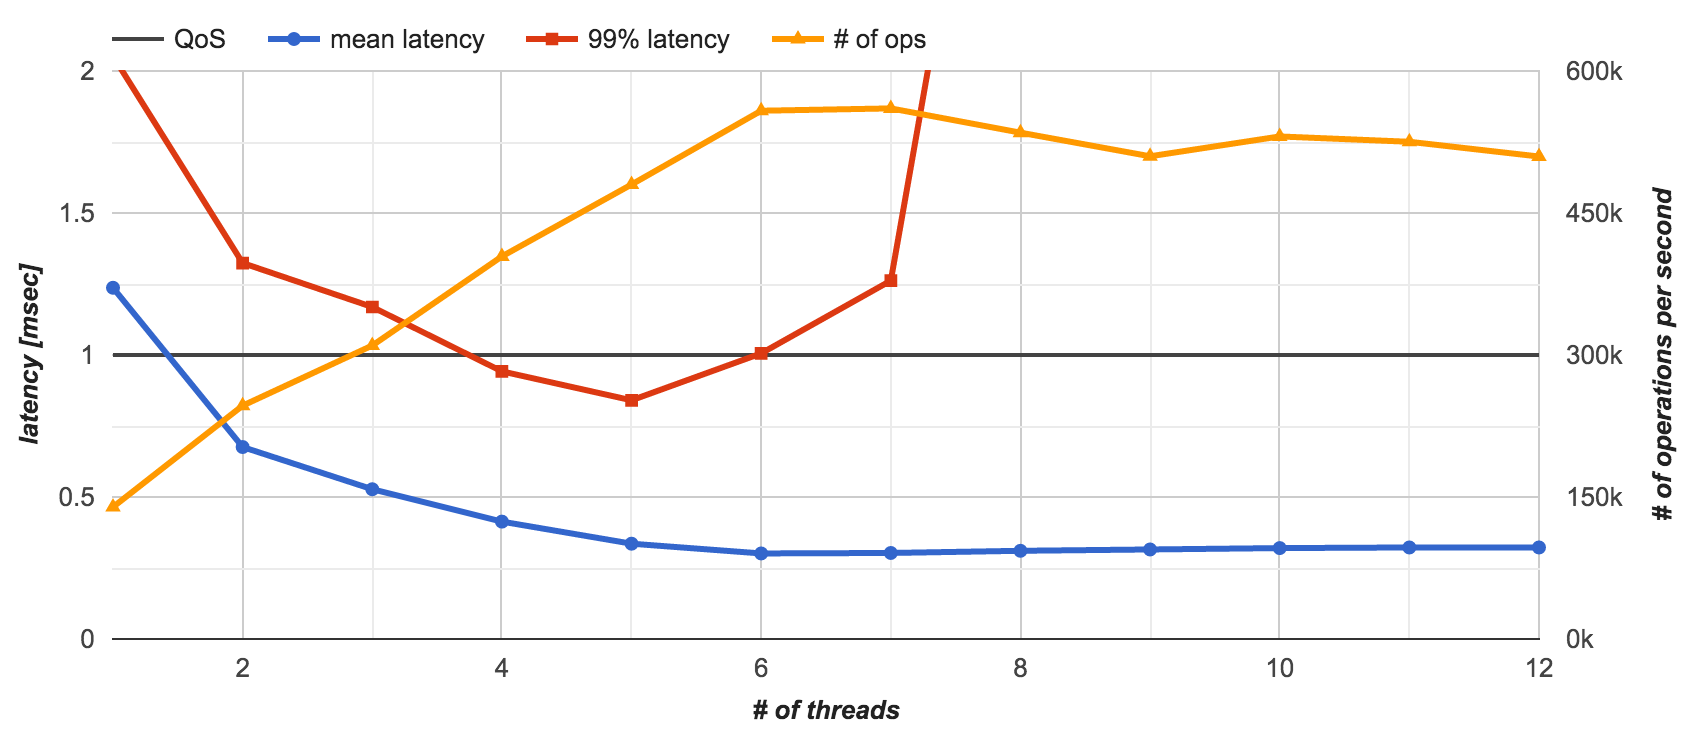
\includegraphics[width=\textwidth]{./res2/m_threads_latency.png}
    \caption{Memcached Threads: Latency \& Throughput vs Number of Threads}
    \label{fig:m_threads_latency.png}
\end{figure}


Figure \ref{fig:m_threads_latency.png} plots the relationship between the number of threads used by Memcached on the horizontal axis, latency on the left vertical and the number of operations on the right vertical.

Mean latency, experiences a sharp decrease between 1 and 2 threads and increases steadily as the number of threads increases beyond 2 threads.
The 99th percentile latency fails to meet the QoS constraints initially between 1 and 2 threads, dropping below the QoS constraint with 3, 4 and 5 threads. However, it climbs beyond the QoS requirements with 6 threads and continues to increase as the number of threads increases.
The number of operations increases sharply between 1 and 2 threads, reaching a maximum of 270k requests per second while decreasing as the number of threads increases.

The performance obtained with increased number of threads does not match our expectations of best performance at 6 threads. However, we can still observe the expected downward shaped parabolic curve the 99th percentile latency plots. Let us examine the CPU utilization to gain a better insight into the problem.


\subsection{CPU Utilization}

Figure \ref{fig:m_threads_cpu} provides the \textit{mpstat} category breakdown of the CPU utilization of Memcached during the benchmark. Note that unattributed utilization accounts for idle time.

\begin{figure}[h]
    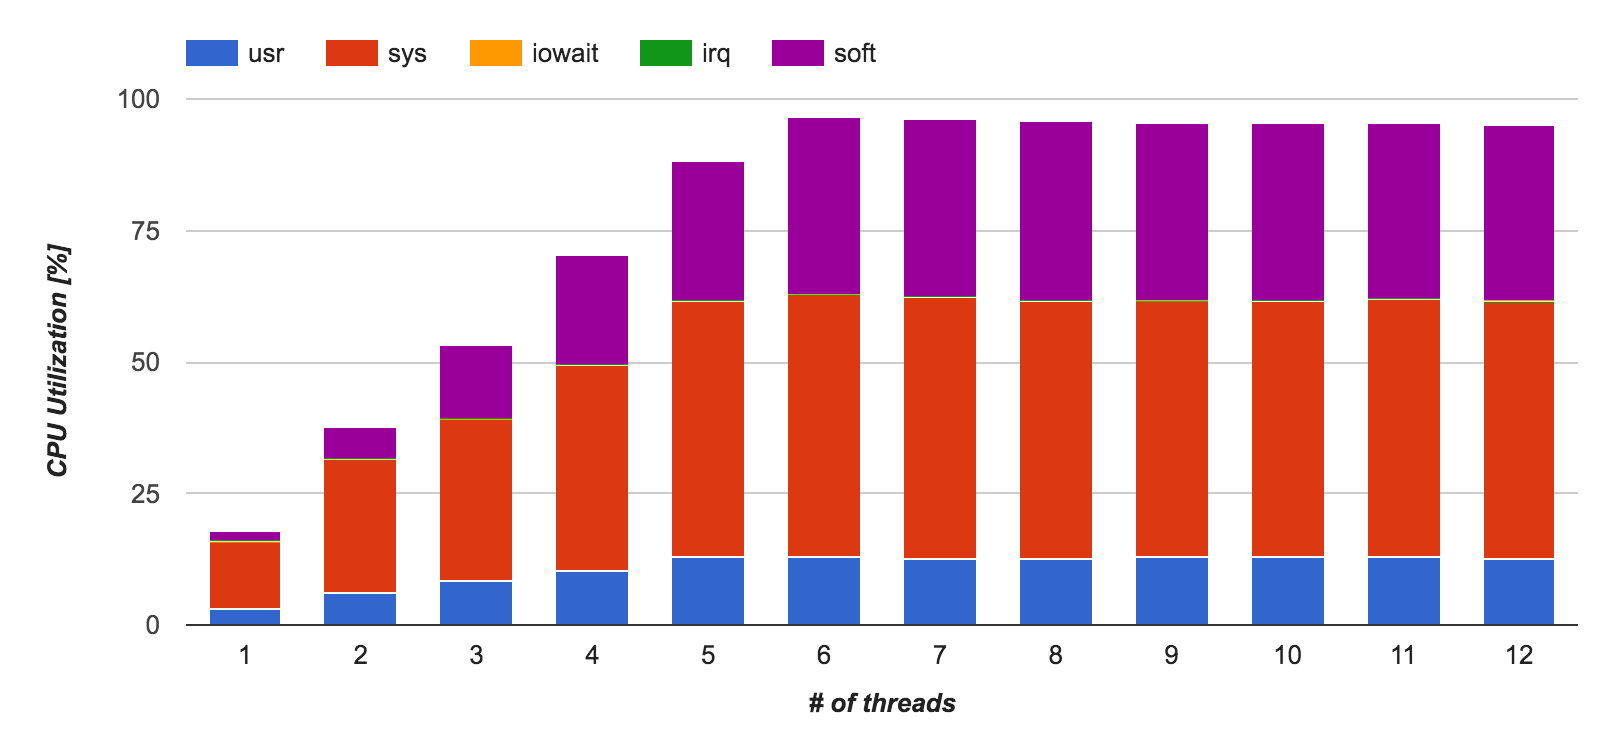
\includegraphics[width=\textwidth]{./res2/m_threads_cpu.png}
    \caption{Memcached CPU Utilization with Multiple Threads}
    \label{fig:m_threads_cpu}
\end{figure}

The CPU utilization of Memcached accounts for a small portion of the total utilization. Initially, with 1 thread Memcached only accounts for 3\% of total utilization. As the number of threads increases, Memcached CPU usage increases too, however, only up to 4 threads at which point it remains constant.
The kernel usage increases with the number of threads and stabilizes at 4 threads with 34\%. An increase in the number of threads does not result in increase in the kernel usage.
Software interrupt CPU usage increases from 2\% to 15\% between 1 and 2 threads and remains stable as the number of threads increases.
Similarly to previous benchmarks, disk IO and hardware interrupts take up insignificant portions of the CPU utilization.

Overall, we can observe that the total CPU utilization reaches at most 65\%. The CPU usage overall does not reflect our expectation of increased CPU usage with more threads. In fact, there is no significant increased utilization with more than 4 threads.

Interestingly, the software interrupt usage only increases between 1 and 2 threads which is contrary to the expectation of a linear increase in interrupt processing with multiple threads. Let us investigate CPU utilization further by focusing on the breakdown of individual CPU usage.

\begin{figure}[h]
    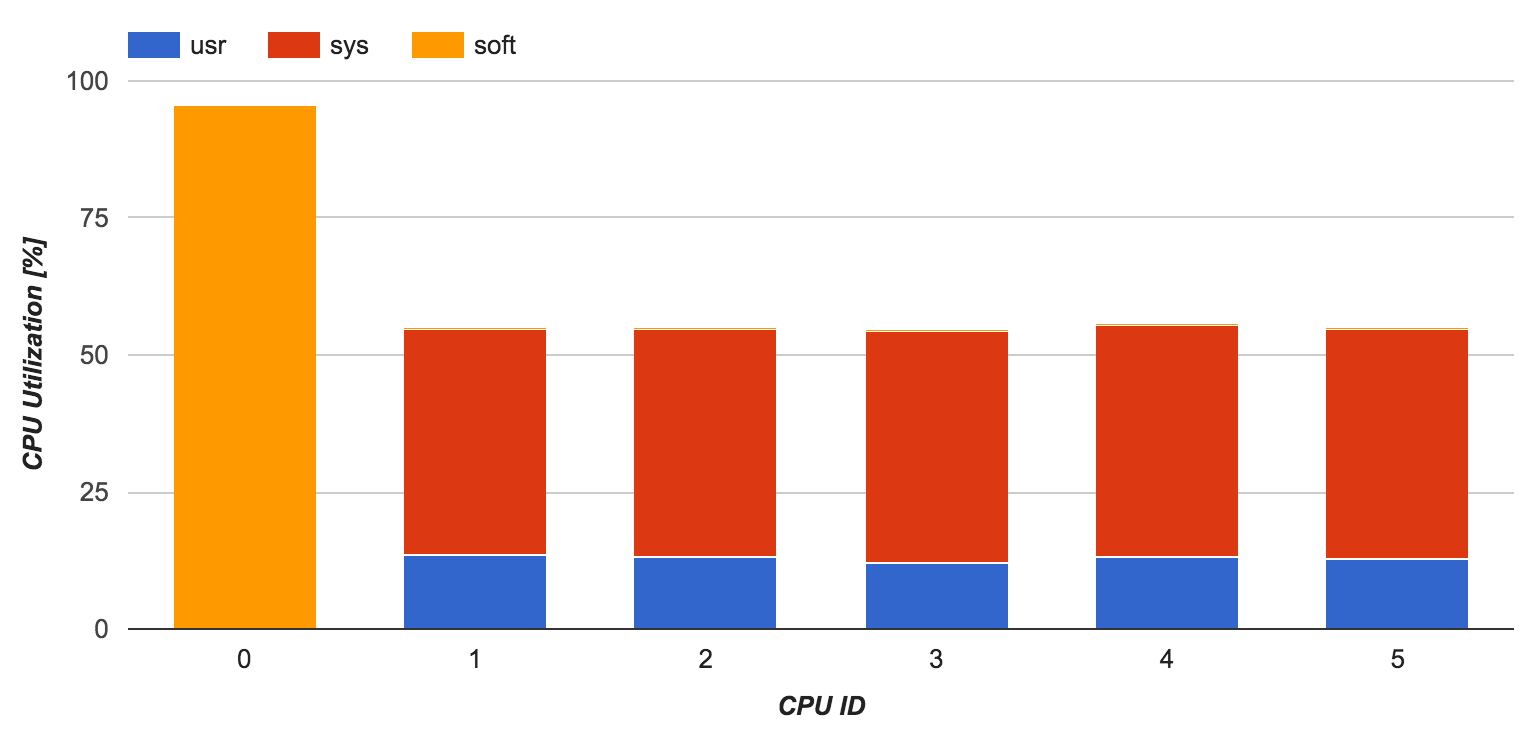
\includegraphics[width=\textwidth]{./res2/m_threads_cpu_individual.png}
    \caption{Memcached CPU Utilization with 6 threads by Individual CPU}
    \label{fig:m_threads_cpu_individual}
\end{figure}

Figure \ref{fig:m_threads_cpu_individual} shows the category breakdown of CPU utilization by each CPU for Memcached with 6 threads. We can observe that CPU 0 is processing all of the software interrupts while the remaining CPUs handle Memcached and the kernel. It is apparent that processing all of the software interrupts on a single CPU cores is a bottleneck in this case as the remaining CPUs are heavily underutilized. This phenomenon can be described as ``load imbalance'' \cite{leverich2014reconciling}. The kernel is responsible for scheduling software interrupt processing and depending on the configuration it may choose to process all interrupts on a single CPU.

\subsection{Threads Conclusion}
In this section, we have explored the impact of threading on Memcached performance. We have reasoned that the best performance will be delivered when running with as many threads as there are CPU cores, however, our benchmarks have showed that this is in fact not the case. Closer inspection of the behavior has shown that the culprit is software interrupt processing on only one CPU core rendering it a bottleneck for the rest of the system. In order to solve this problem, we will examine explicit assignment of IRQ affinity to CPU cores in the next section.


% ________________________________________________________
\section{IRQ Affinity}
\label{sec:m_irq_affinity}
We have shown that increasing the number of threads itself does not result in improved CPU utilization and better Memcached performance. In this section, we focus resolving the problem of software interrupt processing on a single core. In order to resolve the load imbalance, it is important to understand how the kernel determines which CPU is responsible for processing a given interrupt.

Firstly, a request arrives at the network interface controller (NIC). The packet is processed by the NIC and pushed onto a receive queue. Secondly, an interrupt is raised to notify the kernel that an action is required. Thirdly, the kernel receives an interrupt, determines the application level destination of the request and inserts the request into a queue. Memcached utilizes \textit{libevent} API to receive and send requests between the kernel and the application and is bound to the \textit{epoll} socket \cite{zhang2014efficient}. When a request is inserted into the epoll socket, a level triggered software interrupt is fired \cite{blacklibtorque}. Each Memcached thread is awaiting the software interrupt with \textit{epoll wait()} \cite{thongprasit2015toward} and the request is processed. In the case where a software interrupt is being processed on a core different from the recipient application, a context switch is required which contributes to high kernel space CPU utilization observed in previous benchmarks.

Therefore, we can reason distributing software interrupt processing across many CPU cores should lead to improved CPU utilization and improved overall performance in terms of throughput and latency as the overhead of context switching and the single CPU bottleneck are mitigated.

The kernel chooses which CPU core is responsible for processing a request is determined through IRQ Affinity. IRQ Affinity is an assignment of a given queue to a given CPU and the overall process is called IRQ Affinity pinning.

Firstly, let us inspect which IRQ queues are being used by the network interface. We can list the queues our \textit{eth0} interfaces uses with the following command:
\begin{lstlisting}
$ cat /proc/interrupts | grep eth0 | awk '{ print $1 " " $9 }'

81: eth0
82: eth0-TxRx-0
83: eth0-TxRx-1
84: eth0-TxRx-2
85: eth0-TxRx-3
86: eth0-TxRx-4
87: eth0-TxRx-5
\end{lstlisting}

We obtain a mapping of queues to individual Transmit and Receive (TxRx) queues. For each queue id, we can list their respective CPUs responsible for processing the queue. The following script provides us with this information:

\begin{lstlisting}
$ for i in $(seq 81 1 87); do
    echo $i $(cat $/proc/irq/$i/smp_affinity_list);
  done;

81 0-5
82 0-5
83 0-5
84 0-5
85 0-5
86 0-5
87 0-5
\end{lstlisting}

We can observe that all of the queues are bound to all available CPUs (zero indexed). In order to assign a particular core to a given queue, we simply write the index of the CPU to the corresponding queue file. We can assign each queue with a unique core with the following script. Note that we leave \textit{eth0} (queue 81) assigned to all CPUs as we do not want to bind processing of network requests to a specific core, we only want the transmit and receive queues to be bound.

\begin{lstlisting}
$ for i in $(seq 82 1 87); do
    echo $(($i % 6)) > /proc/irq/$i/smp_affinity_list;
  done
\end{lstlisting}

With the transmit and receive queues assigned, we are now in a position to determine the effect of IRQ affinity pinning on Memcached performance. We will be using the same configuration as in Section \ref{sec:memcached-threads} as well as increasing the number of threads linearly.

\subsection{Threads, Latency \& Throughput with IRQ pinned}

\begin{figure}[h]
    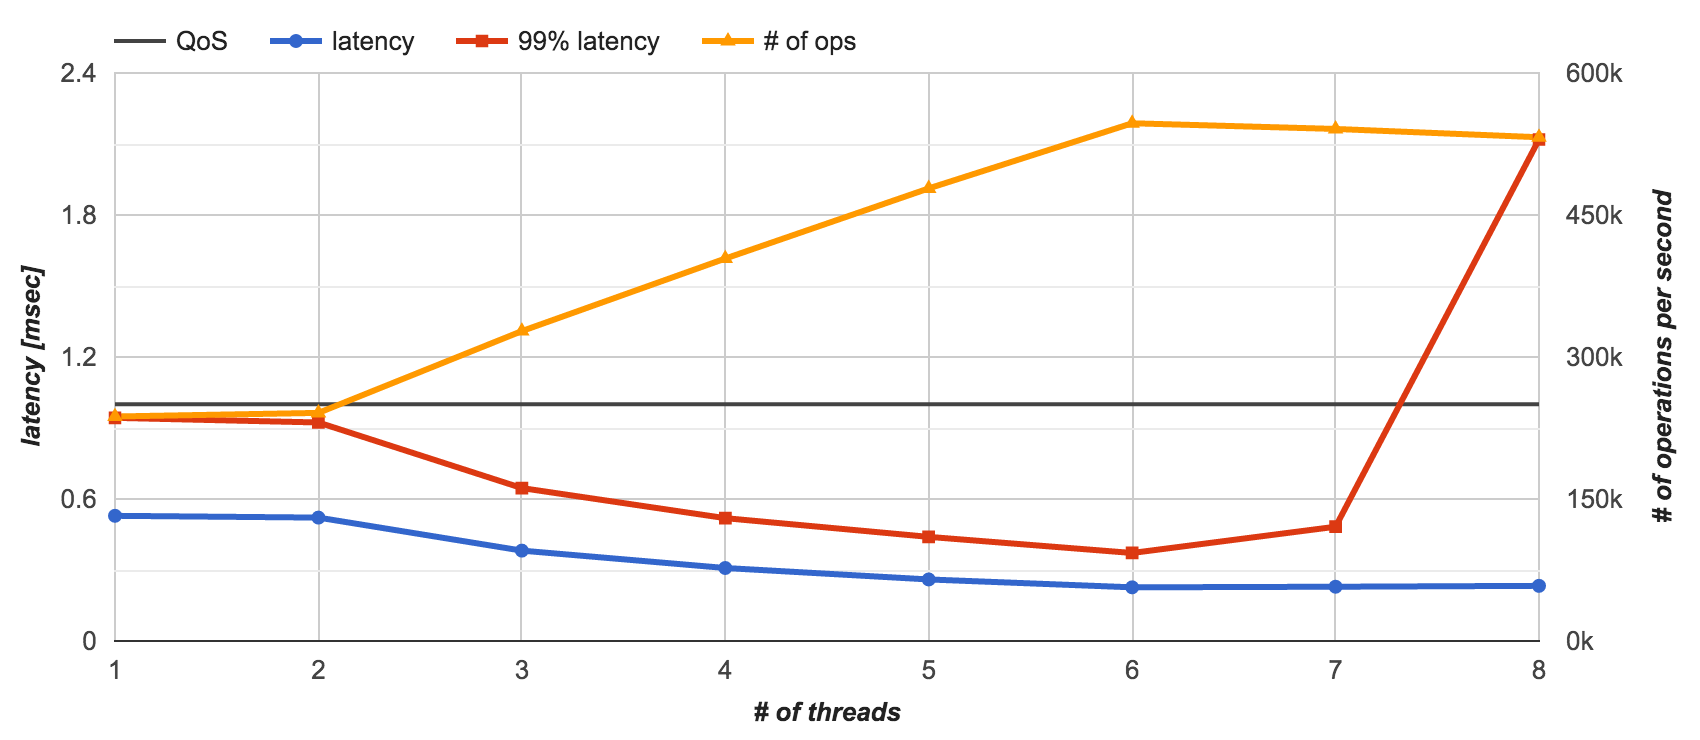
\includegraphics[width=\textwidth]{./res2/m_threads_irq_latency.png}
    \caption{Memcached Latency \& Throughput vs Threads with IRQ Affinity pinned to distinct cores}
    \label{fig:m_threads_irq_latency}
\end{figure}

Figure \ref{fig:m_threads_irq_latency} plots the relationship between latency on the left vertical axis, number of operations per second on the right vertical axis and the number of threads on the horizontal axis.

The mean latency decreases as we increase the number of threads and flattens out at 0.23ms at 6 threads or more. Tail latency, the 99th, decreases as we increase the number of threads. It reaches a minimum of 0.37ms, well within our QoS, at 6 threads and begins to increase as threads increase further. There is a sharp increase between 7 and 8 threads bringing it outside of our QoS. The number of operations per second remains constant between 1 and 2 threads at 240k requests per second. As the number of threads increases, so does throughput. In fact, throughput increases linearly between 2 and 6 threads and peaks at 546k requests per second. Throughput decreases slowly as the number of threads increases beyond 6.

Firstly, throughput improved drastically. In the peaks, we are able to achieve 546k requests per second with IRQ pinned compared to 264k requests previously. According to expectation, throughput is maximized with as many threads as CPU cores. Additionally, we can see throughput decline with more threads than CPU cores as context switching overhead increases.

Secondly, the 99th percentile latency has decreased significantly. With six or less threads, we are now able to achieve the required QoS. Additionally, the 99th percentile latency reaches a minimum with 6 threads providing the best combination of low latency and highest throughput. This is according to our expectation.

\subsection{CPU Utilization with IRQ pinned}

\begin{figure}[h]
    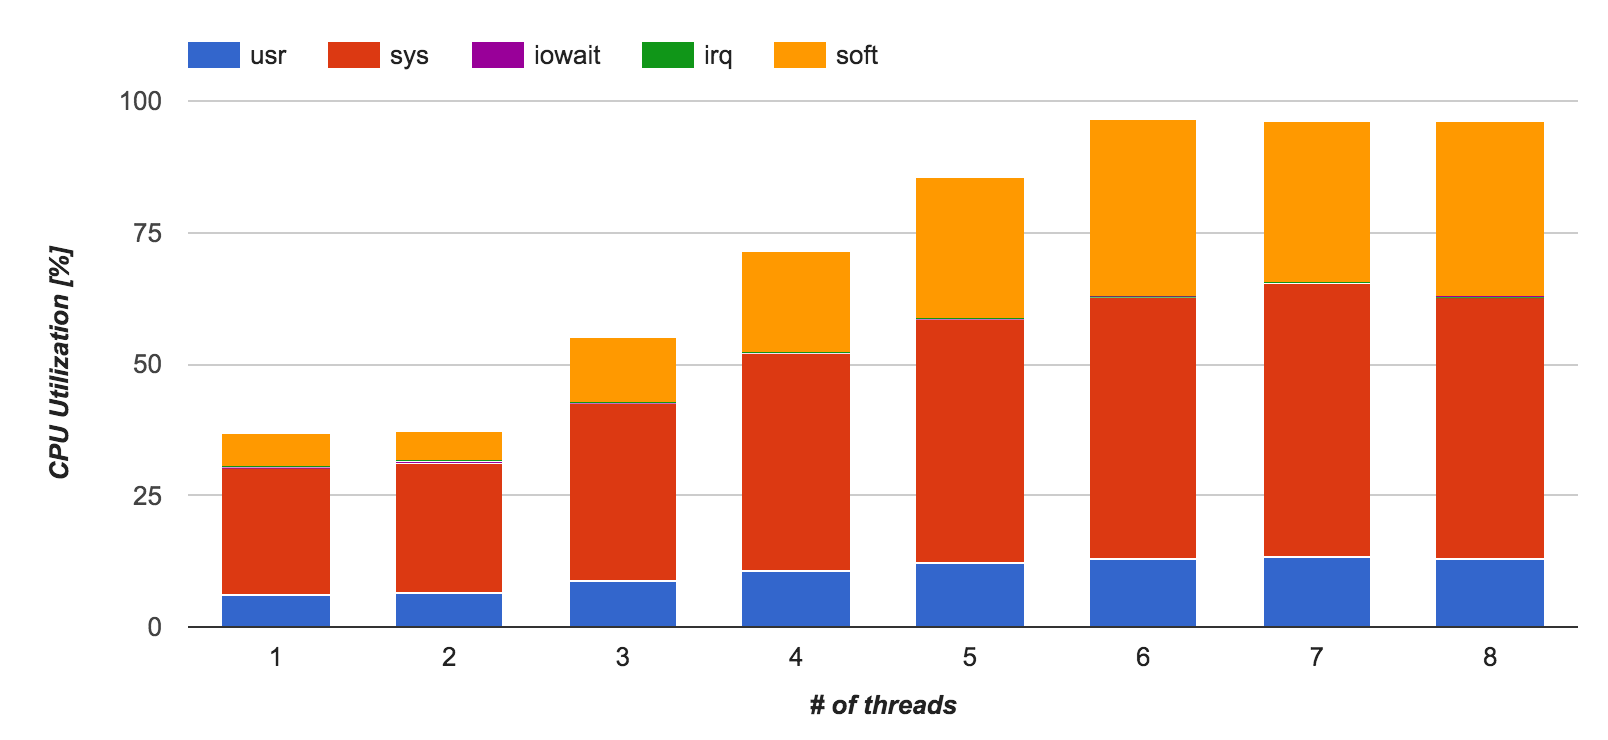
\includegraphics[width=\textwidth]{./res2/m_threads_irq_cpu.png}
    \caption{Memcached CPU Utilization with IRQ Affinity pinned}
    \label{fig:m_threads_irq_cpu}
\end{figure}

Figure \ref{fig:m_threads_irq_cpu} outlines the CPU utilization with IRQ Affinity pinned. The overall ratio of \textit{usr}, \textit{sys} and \textit{soft} remains the same, however, we can observe that as we increase the number of threads the total utilization increases. We achieve near 100\% utilization across all CPUs. Furthermore, CPU utilization breakdown does not change with more than 6 threads. This is reasonable as we are constrained by the number of cycles available to us, more Memcached threads are constrained to the same number of cycles while also incurring a context switching overhead. Therefore, more CPU threads than CPU cores do not result in better performance.

\begin{figure}[h]
    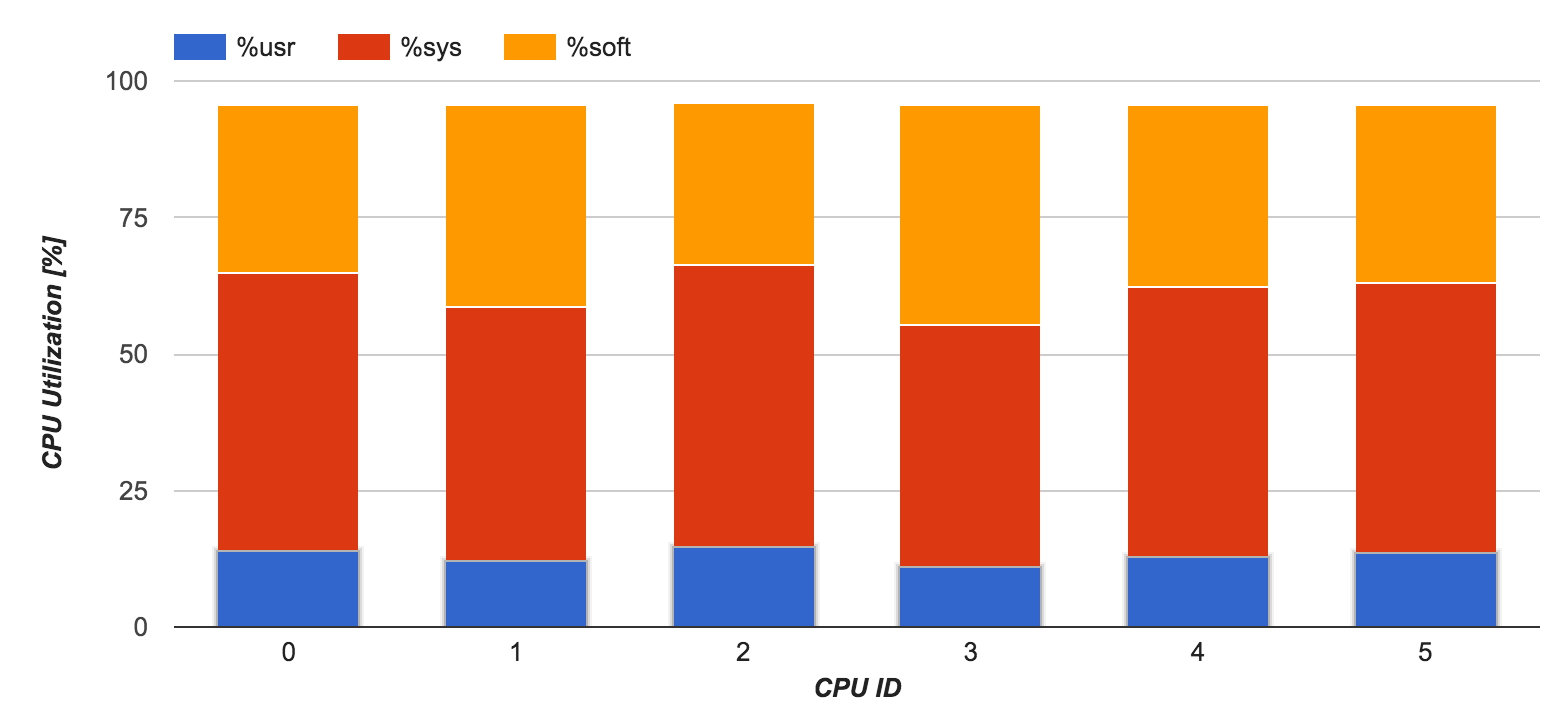
\includegraphics[width=\textwidth]{./res2/m_threads_irq_cpu_individual.png}
    \caption{Memcached with 6 threads - Individual CPU utilization}
    \label{fig:m_threads_irq_cpu_individual}
\end{figure}

Let us consider individual CPU utilization breakdown with 6 threads. Figure \ref{fig:m_threads_irq_cpu_individual} outlines the utilization categories. We can observe that all cores are nearly 100\% utilized as well as all cores participate in software interrupt processing. Utilization of each core is not the same, however. This can be due to a range of factors including given load on each Memcached thread as well as interference from kernel's memory management. Memcached also spawns an additional thread for load balancing purposes \cite{solarflarememcached} which can cause interference in the individual load. This topic will be further examined in the following section.


\subsection{IRQ Conclusion}
We have shown that setting IRQ affinity to individual cores drastically improves performance of Memcached. Throughput has increased more than two fold while the 99th percentile latency decreased. Distribution of work across the CPU cores has improved and we have been able to fully utilize all of the cores available to us. For the rest of this chapter, all benchmarks executed will be considered with IRQ affinity set distinct cores.

% ________________________________________________________

\section{Thread pinning}
\label{sec:thread-pinning}
We now turn our attention to individual threads of Memcached. Thread pinning is the process of assigning a \textit{set\_irq\_affinity} to each individual thread. As suggested by Leverich and Kozyrakis, "pinning memcached threads to distinct cores greatly improves load balance, consequently improving tail latency." \cite{leverich2014reconciling} Furthermore, ``While it is not strictly necessary, it may be additionally beneficial to pin every Memcache worker thread onto a single CPU to further improve performance by minimising cache pollution.'' \cite{solarflarememcached} Therefore, we will investigate thread pinning and their impact on performance.

Firstly, it is important to understand how the kernel determines which core a process/thread will run on. It is the responsibility of the \textit{scheduler} to maintain CPU cores busy and schedule work \cite{siddha2005chip}. As such, the scheduler decided which core an application should be scheduled and executed on. As such, a scheduler aims to optimize for a given metric, such as utilization, priority or aims to avoid starvation. By default, when a new process is started it can be scheduled on any CPU core. As a result, the scheduler may choose to schedule multiple threads on the same CPU core. In order to explicitly prevent such behavior, we can set a distinct core for each thread using the \textit{taskset} utility. We can discover the CPU affinity of a given process through the following command where \textit{pid} is the process identifier.

\begin{lstlisting}
    taskset -p <pid>
\end{lstlisting}


"A Memcache instance started with n threads will spawn n + 1 threads of which the first n are worker threads and the last is a maintenance thread used for hash table expansion under high load factor." \cite{solarflarememcached}. We can discover memcached threads used for request processing using the following command where \textit{tid} is the thread id discovered previously \cite{solarflarememcached}.
\begin{lstlisting}
    ps -p <memcache-pid> -o tid= -L | sort -n | tail -n +2 | head -n -1
\end{lstlisting}

For this benchmark, we use the same configuration as in previous sections. Tables \ref{tab:m_threads_memtier} and \ref{tab:m_threads_memcached} provides the complete configuration.

\subsection{Latency \& Throughput vs Threads}

\begin{figure}[h]
    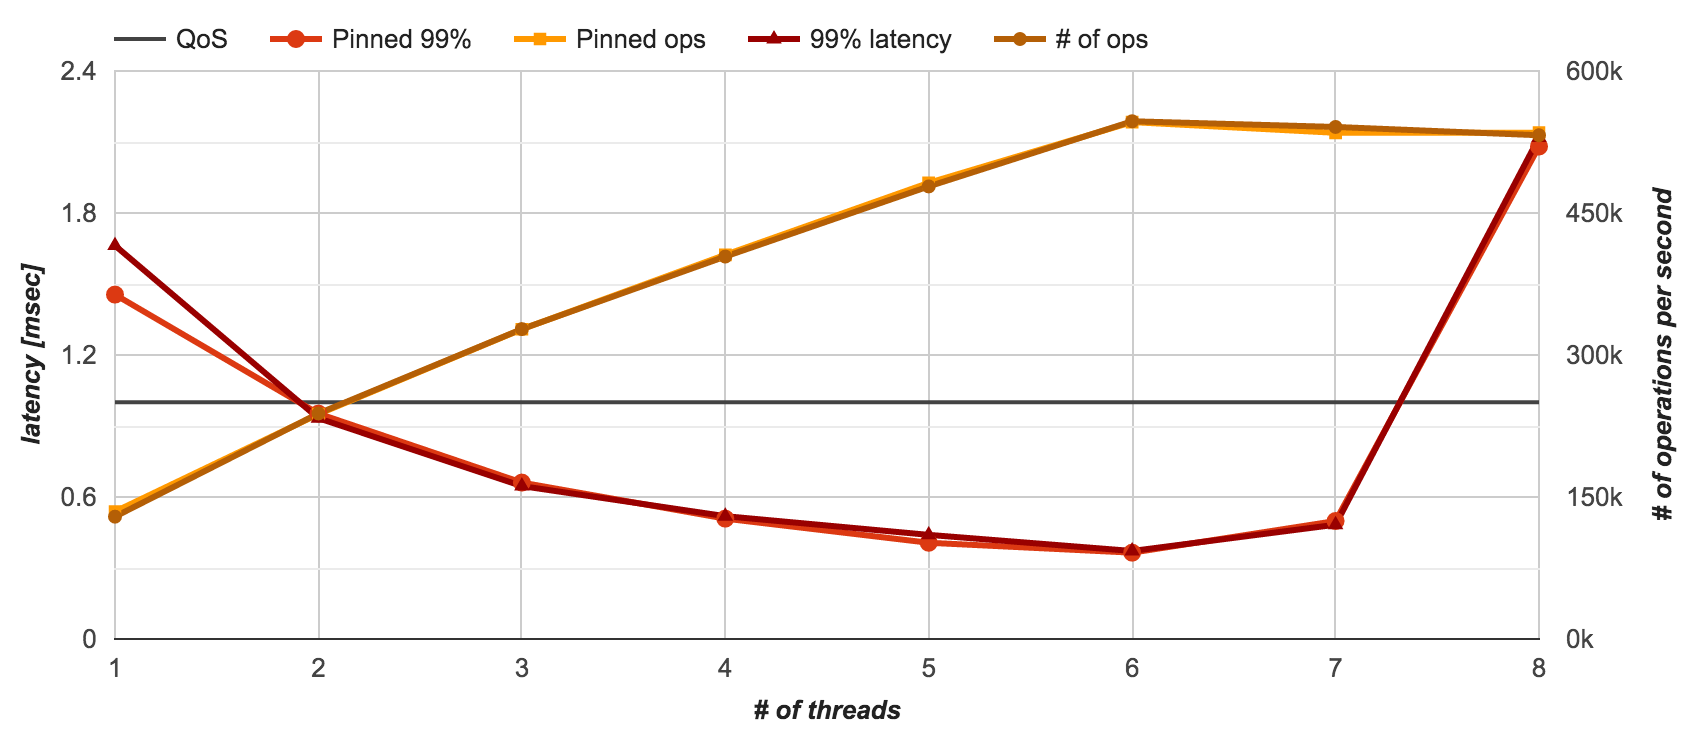
\includegraphics[width=\textwidth]{./res2/m_pinning_latency.png}
    \caption{Memcached Latency \& Throughput vs Threads: Comparison of pinned threads (labeled: \textit{Pinned}) vs unpinned threads}
    \label{fig:m_pinning_latency}
\end{figure}

Figure \ref{fig:m_pinning_latency} presents a comparison of Memcached with pinned threads against unpinned threads. Overall, thread pinning appears to be no significant change in performance with threads pinned. In the case of Memcached with 1 thread, there appears to be an improvement in the tail latency, however, the QoS constraint is still violated.

We expected to see an improvement in tail latency or throughput. However, as other research suggests the improvement may only be observable in environments with a higher number of cores and/or in environments with shared workloads and only a fixed number of cores dedicated to Memcached \cite{solarflarememcached}.

\subsection{CPU Utilization}

\begin{figure}[h]
    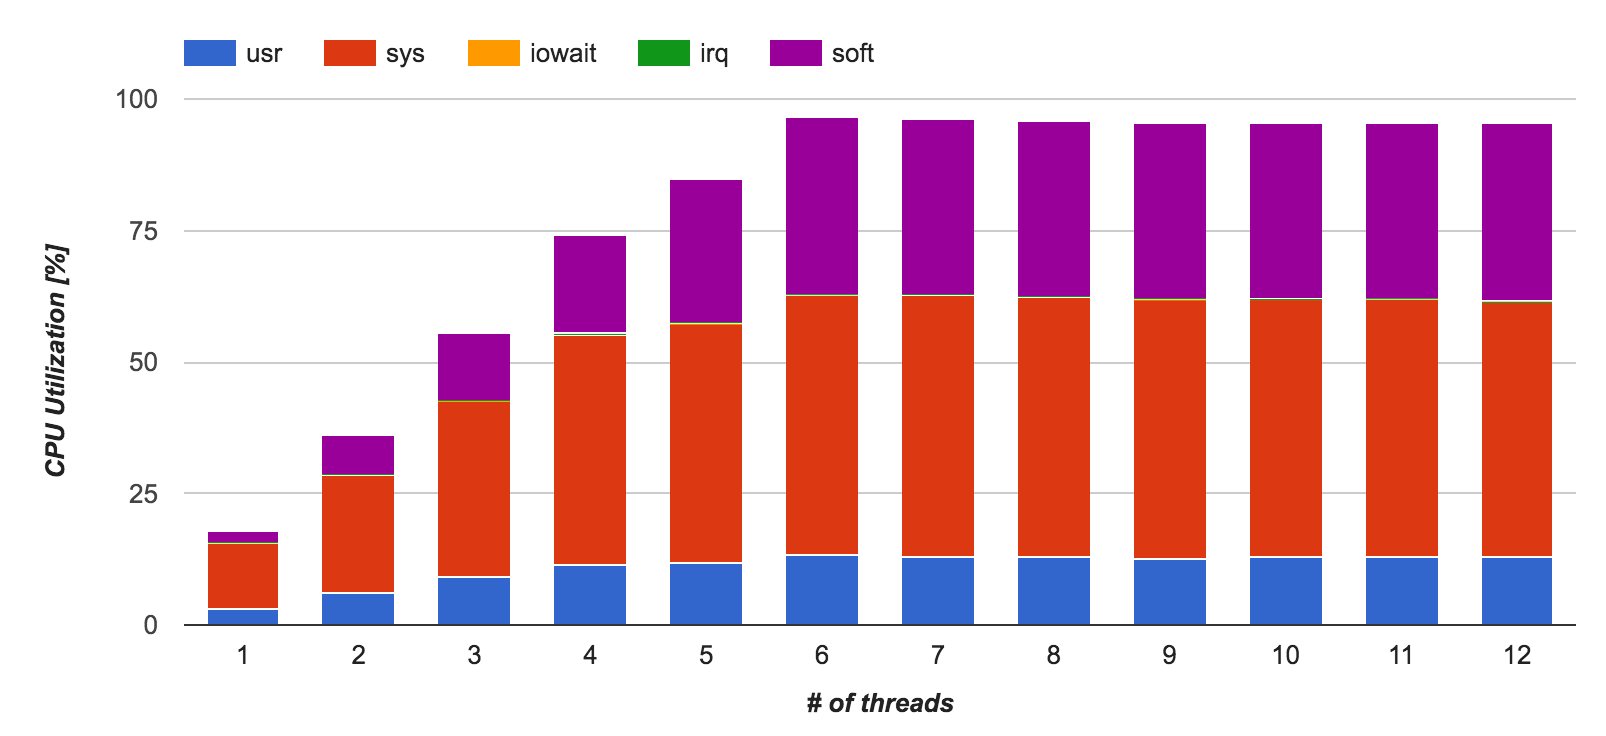
\includegraphics[width=\textwidth]{./res2/m_pinning_cpu.png}
    \caption{Pinned Memcached CPU Utilization}
    \label{fig:m_pinning_cpu}
\end{figure}

Figure \ref{fig:m_pinning_cpu} presents the overall CPU Usage with Memcached threads pinned. The CPU Utilization of pinned threads is nearly identical to unpinned threads presented in Figure \ref{fig:m_threads_cpu}.

\begin{figure}[h]
    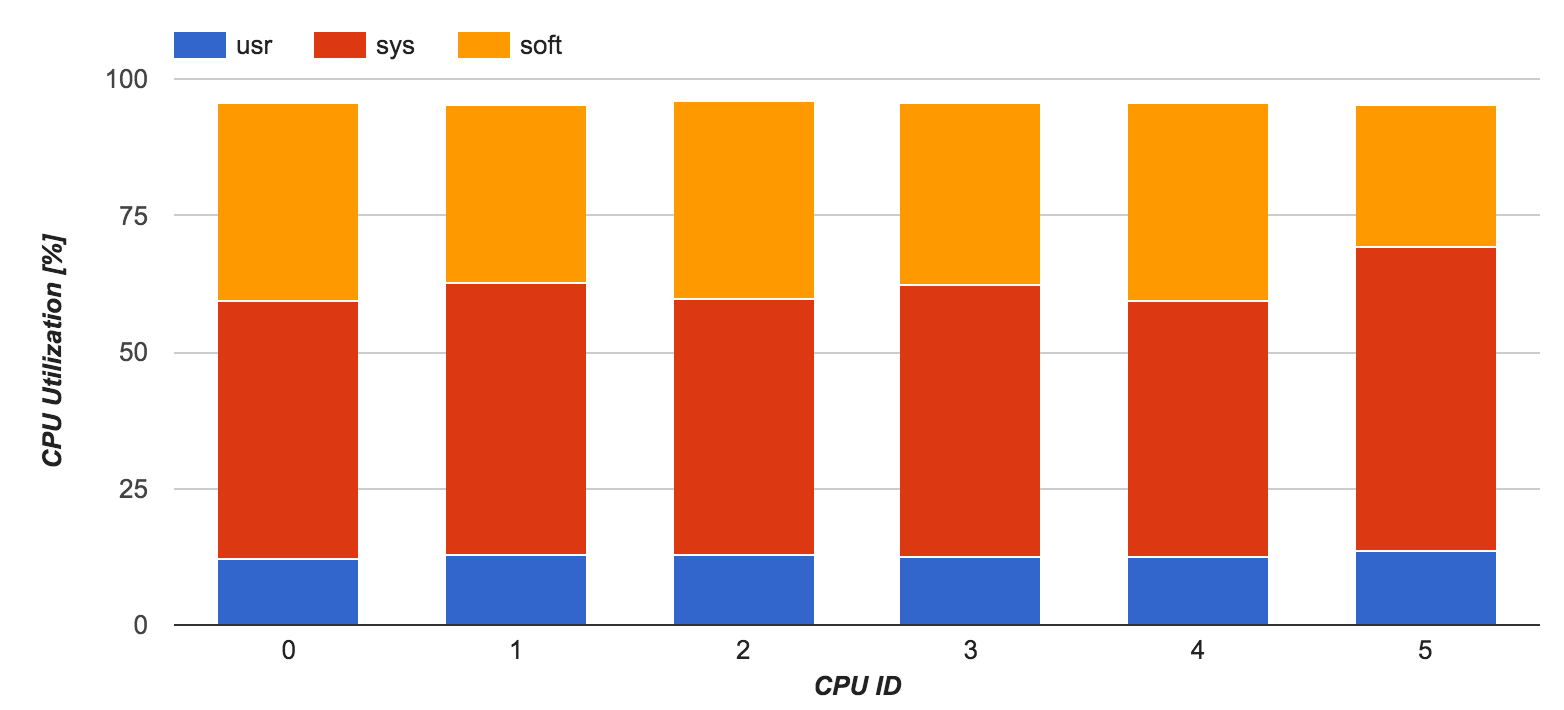
\includegraphics[width=\textwidth]{./res2/m_pinning_cpu_individual.png}
    \caption{Pinned Memcached Individual CPU Utilization with 6 threads}
    \label{fig:m_pinning_cpu_individual}
\end{figure}

Figure \ref{fig:m_pinning_cpu_individual} plots the individual CPU usage breakdown. With thread pinning, we can observe a more evenly balanced distribution of CPU utilization as opposed to Figure \ref{fig:m_threads_irq_cpu_individual}.

\subsection{Thread Pinning Conclusion}
We have shown that thread pinning, in our benchmark, does not impact Memcached performance negative nor does it have a positive impact. CPU Utilization remains the same with thread pinning, however, the distribution of user, kernel and software interrupt processing is more balanced. Our findings are not consistent with findings reported by Leverich \& Kozyrakis \cite{leverich2014reconciling}. This may be due to scheduling policy inconsistency of the systems. However, it has been suggested that thread pinning reduces interference and therefore in subsequent benchmarks we will pin Memcached threads unless otherwise stated.


% ________________________________________________________

\section{Group Size}
In this section, we focus on the effect of connections on the performance of the cache. Memcached provides a configuration option \textit{-R} to set the group size in the connection management policy of Memcached. The group size defines the ``maximum number of requests per event, limits the number of requests processed for a given connection to prevent starvation (default: 20)'' \cite{interactive2006memcached} and has a maximum value of 320 enforced in the implementation of Memcached \cite{blake54does}. This in effect means the number of requests processed from a single connection before memcached switches to a different connection to enforce a fairness policy.

In this benchmark, we focus on the effect of the group size on a Memcached deployment with 6 threads - the best configuration found so far. The benchmark increases the group size linearly in increments of 20 starting at 20 up to the maximum. The table below summarizes the Memcached and Memtier configurations used in this benchmark.

\begin{table}[h!]
\centering
\begin{tabular}{| c c c | c c c |}
 \hline
 \multicolumn{3}{|c|}{Memcached} & \multicolumn{3}{|c|}{Memtier} \\
 \hline
 Flag & Explanation & Value & Flag & Explanation & Value \\ [0.5ex]
 \hline\hline

 -d & Daemon Mode & true        & -s & Server & nsl200 \\
 -p & Port number & 11120       & -p & Port number & 11120 \\
 -t & Thread count & 6          & -c & Conn. Count & 7 \\
 -m & Memory & 6144 (6GB)       & -t & Thread Count & 3 \\
 -R & Group Size & [20..320]    & --key-minimum & Min Key & 1 \\
 & &                            & --key-maximum & Max Key & 100m \\
 & &                            & --random-data & Gen random & true \\
 & &                            & --data-size & Data Size & 64 \\

 \hline

\end{tabular}
\caption{Group Size benchmark configuration}
\label{tab:m_threads_memcached}
\end{table}


\subsection{Latency \& Throughput}

\begin{figure}[h]
    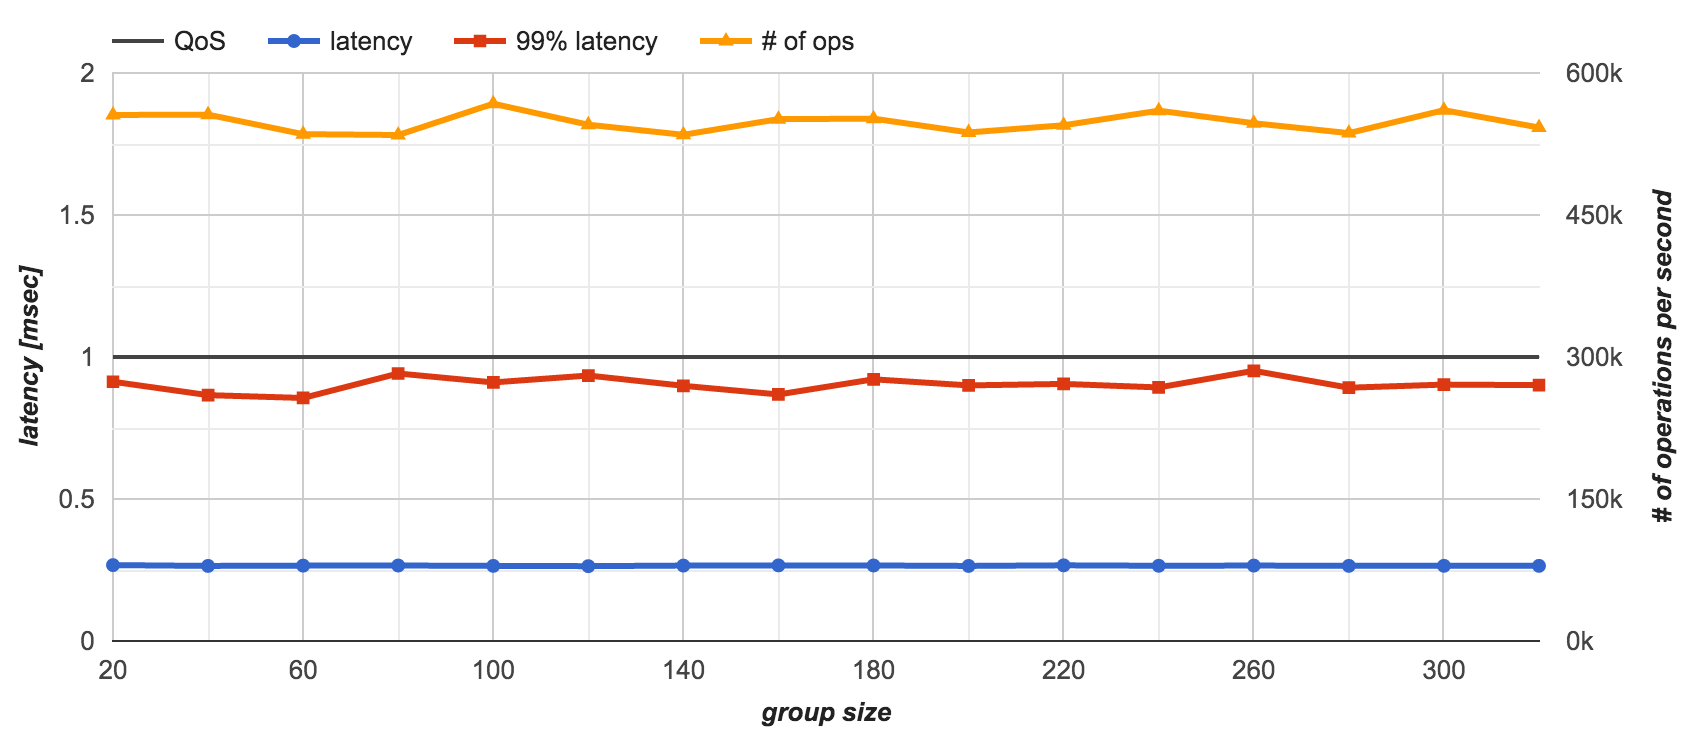
\includegraphics[width=\textwidth]{./res2/m_group_size_latency.png}
    \caption{Latency \& Throughput vs Memcached Group Size }
    \label{fig:m_group_size_latency}
\end{figure}

Figure \ref{fig:m_group_size_latency} plots the relationship between group size, latency and throughput. Overall, there is very little difference in the performance at various group sizes. The throughput remains constant at 545k requests per second with tail latency at 0.35ms. The mean latency remains constant too at 0.22ms.

\subsection{CPU Utilization}

\begin{figure}[h]
    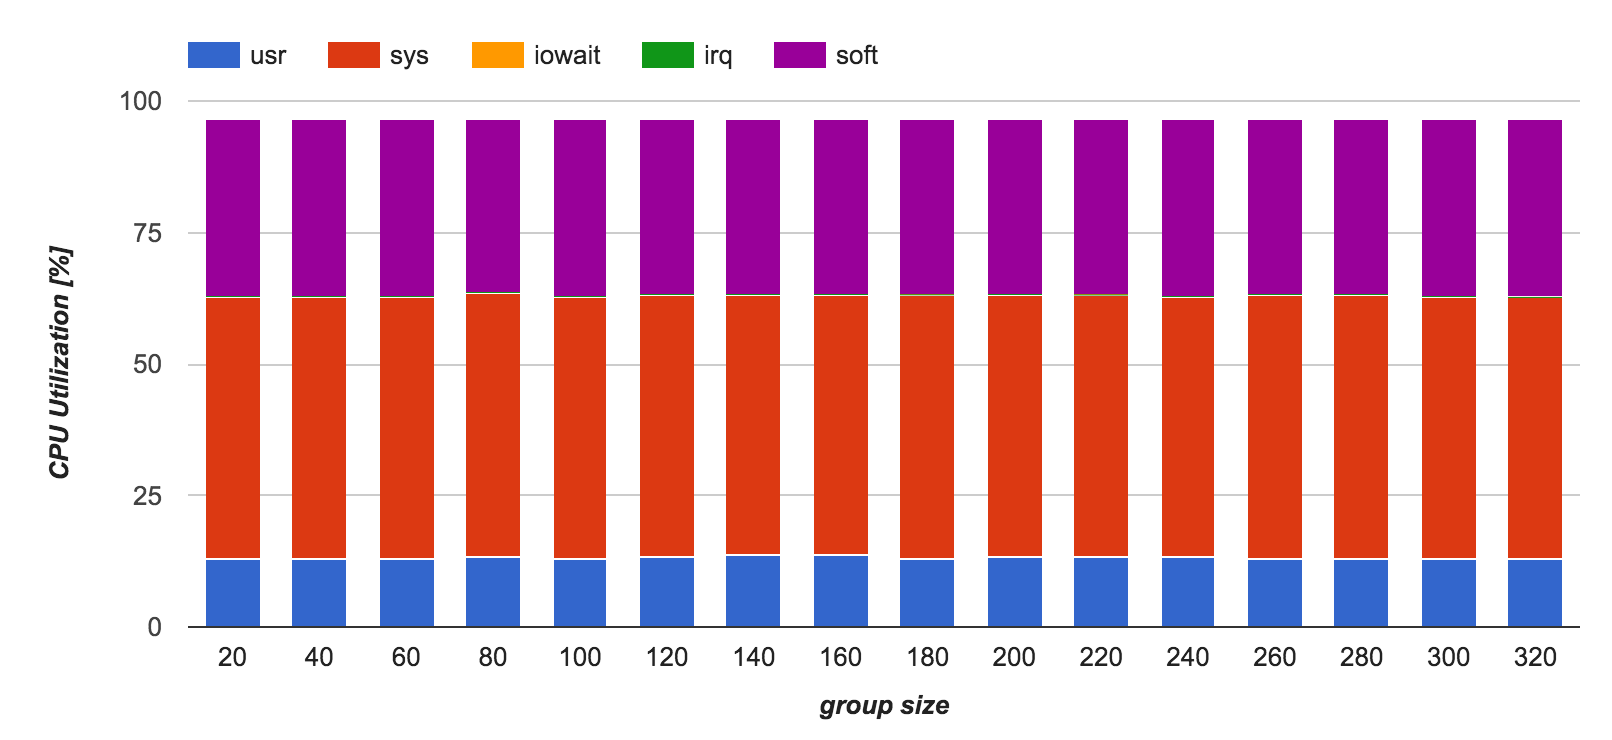
\includegraphics[width=\textwidth]{./res2/m_group_size_cpu.png}
    \caption{CPU Utilization vs Memcached Group Size}
    \label{fig:m_group_size_cpu}
\end{figure}

Figure \ref{fig:m_group_size_cpu} plots the CPU utilization reported by \textit{mpstat}. We can observe that group size does not have any impact on the distribution of CPU utilization, nor does it impact the total utilization of the CPU.

\subsection{Group Size Conclusion}
In our benchmarks, we have observed that group size does not have any impact on the overall performance of Memcached. We have used 147 simultaneous connections in our benchmark, however, a smaller number of connections with higher throughput may be required to effectively exploit the group size. The benchmark setup does not allow us to generate a high enough load from a singular connection and therefore we are unable to replicate the results obtained by Blake and Saidi \cite{blake54does}.


% ---------------------------------------------------------------
\section{Multiple Instances}
\label{sec:m_multiple_instances}
In this section, we focus on a scenario with multiple separate Memcached instances (processes). In a production deployment, it may be desirable to logically split a Memcached deployment into multiple instances. This decision can be driven by application isolation, ability to migrate deployments independently or simply running multiple applications on the same server.

In the context of this paper, we consider an ``instance'' to be an application with an isolated view of the rest of the system. Therefore, when referring to an instance, we make the assumption that multiple instances cannot communicate with each other and more generally the instance makes no assumptions about the rest of the system or other applications on the same system.

We have previously concluded that the best performance is achieved with as many threads/processes as there are CPU cores. In this section, we build on top of this observation and design the benchmark with at most as many threads/processes as there are CPU cores.

Given the hardware configuration of this paper with 6 CPU cores, we can construct multiple scenarios of instances on the server. Table \ref{tab:m_instances_config} outlines the configuration scenarios with respect to the number of instances, threads and the total number of threads/processes. Note that the scenario with only 1 instance corresponds the previously explored scenario and serves as a baseline for comparison.

\begin{table}[h!]
\centering
\begin{tabular}{| c c c |}
 \hline
 Number of Instances & Threads per Instance & Total threads/processes \\ [0.5ex]
 \hline\hline

 1 & 6 & 6 \\
 2 & 3 & 6 \\
 3 & 2 & 6 \\
 6 & 1 & 6 \\

 \hline

\end{tabular}
\caption{Configuration Scenarios with at most 6 threads/processes on the server}
\label{tab:m_instances_config}
\end{table}

For the purposes of this section, we will use a modified configuration for the workload generating clients. We have previously observed that Memtier with 3 threads and 7 connections provides a sufficient workload to saturate the object cache, however, achieves a tail latency close to 0.4ms. We increase the number of connections in this benchmark to 30 in order to gain flexibility for workload partitioning. This is necessary as 21 connections cannot be partitioned evenly across 6 instances due to indivisibility. Instead, we choose 30 connections per each workload generating host. The direct consequence of increasing the number of connections is expected to be an increase in the tail latency. Throughout the benchmark, we continue to target the required QoS.

\begin{table}[h!]
\centering
\begin{tabular}{| c c c |}
 \hline
 Number of Instances & Threads per Instance & Memory per Instance \\ [0.5ex]
 \hline\hline

 1 & 6 & 6GB \\
 2 & 3 & 3GB \\
 3 & 2 & 2GB \\
 6 & 1 & 1GB \\

 \hline

\end{tabular}
\caption{Memcached configuration for multiple instances}
\label{tab:m_instances_memcached_conf}
\end{table}

Table \ref{tab:m_instances_memcached_conf} outlines the Memcached configuration at individual instance configurations. Note that the total amount of memory allocated remains constant. Additionally, when there are multiple threads per instance, each thread is pinned to an individual core.

\begin{table}[h!]
\centering
\begin{tabular}{| c c c c c|}
 \hline
 Number of Instances & Threads & Connections & Key Maximum & Total Dataset\\ [0.5ex]
 \hline\hline

 1 & 6 & 5 & 10 million & 6.4 GB \\
 2 & 3 & 5 & 5 million & 6.4 GB \\
 3 & 2 & 5 & 3.3 million & 6.4 GB \\
 6 & 1 & 5 & 1 million & 6.4 GB \\

 \hline

\end{tabular}
\caption{Memtier configuration for multiple instances}
\label{tab:m_instances_memtier_conf}
\end{table}

Table \ref{tab:m_instances_memcached_conf} outlines the Memtier configuration at individual instance configurations. The total size of the dataset remains constant, however, the maximum key is lowered to allow for the increased number of instances. Furthermore, each workload generating host will execute as many instances of Memtier as there are corresponding instances of Memcached effectively spreading the load evenly across each individual instance.

\subsection{Latency \& Throughput vs Instances}

\begin{figure}[h]
    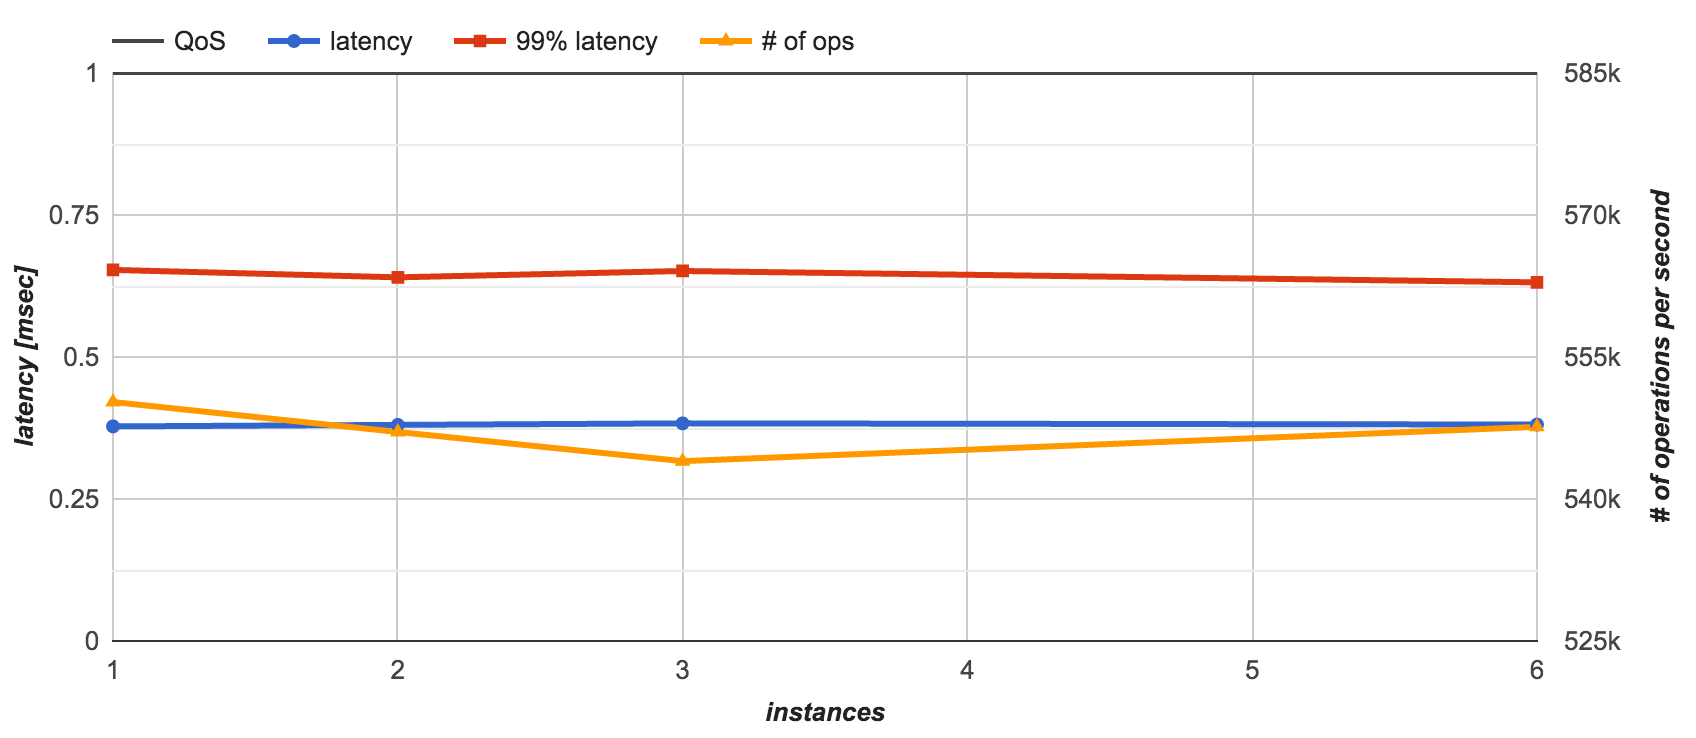
\includegraphics[width=\textwidth]{./res2/m_instances_latency.png}
    \caption{Multiple Instances: Latency \& Throughput vs Number of instances. Note the scale of the right vertical axis starts at 525k.}
    \label{fig:m_instances_latency}
\end{figure}

Figure \ref{fig:m_instances_latency} plots mean latency, 99th percentile latency and throughput as the number of instances is increased. Mean latency and 99th percentile latency remain nearly constant as the number of instances increases. There is a very slight increase in latency at 3 instances, however, it is rather insignificant with respect to the scale. Throughput is maximized with only 1 instance and reaches a minimum at 3 instances, however, the difference is rather insignificant relative to the scale.

\subsection{CPU Utilization vs Instances}

\begin{figure}[h]
    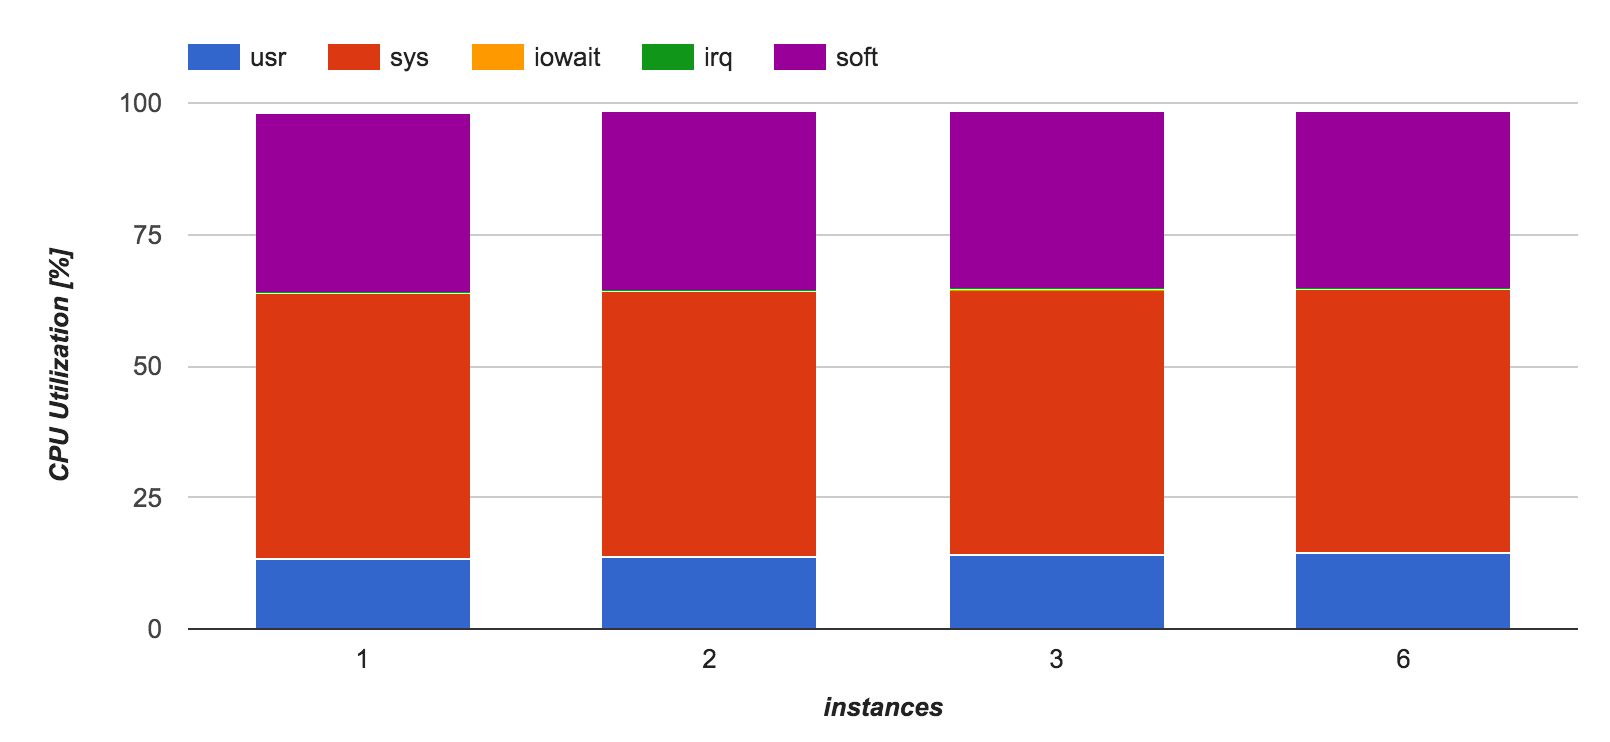
\includegraphics[width=\textwidth]{./res2/m_instances_cpu.png}
    \caption{CPU Utilization with Multiple Instances}
    \label{fig:m_instances_cpu}
\end{figure}

Figure \ref{fig:m_instances_cpu} plots the CPU utilization with multiple instances. We can observe that the number of instances does not impact the total utilization nor does it impact the breakdown of individual category utilization.

\subsection{Multiple Instances Conclusion}
From the benchmark, we can conclude that multiple instances with proportionate allocation of resources do not incur any significant penalties in terms of performance. We have observed a slight decrease in throughput and increase in 99th percentile latency with a shared workload of 3 instances at 2 threads each. However, the relative scale of the change as well as the limited number of shared workload scenarios do not provide sufficient evidence to reach a conclusion.


% ---------------------------------------------------------------
\section{Object Size}
\label{sec:m_object_size}
In this section, we turn our focus away from optimizing the performance of the cache itself onto the the effect of the data stored in the cache. We focus on the object size, the data stored in the cache. In particular, we focus on the scalability of Memcached with larger objects. It has been reported that ``object size distribution has a large impact on system behavior'' \cite{lim2013thin}.

In this benchmark, we utilize the same configuration as in Section \ref{sec:m_multiple_instances}, specifically we consider single instance Memcached with 6 threads since we found multi-instance setup of Memcached does not improve performance. On the client workload generation side, we reuse our configuration with 30 connections per each client host. We maintain the client side dataset constant at 6.4 GB, however, we adjust the maximum key based on the data size in order to maintain the same key range to data size ratio. Table \ref{tab:m_object_size_config} outlines the configuration details used for this benchmark.

\begin{table}[h!]
\centering
\begin{tabular}{| c c c | c c c |}
 \hline
 \multicolumn{3}{|c|}{Memcached} & \multicolumn{3}{|c|}{Memtier} \\
 \hline
 Flag & Explanation & Value & Flag & Explanation & Value \\ [0.5ex]
 \hline\hline

 -d & Daemon Mode & true        & -s & Server & nsl200 \\
 -p & Port number & 11120       & -p & Port number & 11120 \\
 -t & Thread count & 6          & -c & Conn. Count & 5 \\
 -m & Memory & 6GB              & -t & Thread Count & 6 \\
 & &                            & --key-minimum & Min Key & 1 \\
 & &                            & --key-maximum & Max Key & 6.4GB / data\_size \\
 & &                            & --random-data & Gen random & true \\
 & &                            & --data-size & Data Size & [64B..512KB] \\

 \hline

\end{tabular}
\caption{Memcached \& Memtier configuration for Object Size benchmark}
\label{tab:m_object_size_config}
\end{table}

\subsection{Latency \& Throughput vs Object Size}

\begin{figure}[h]
    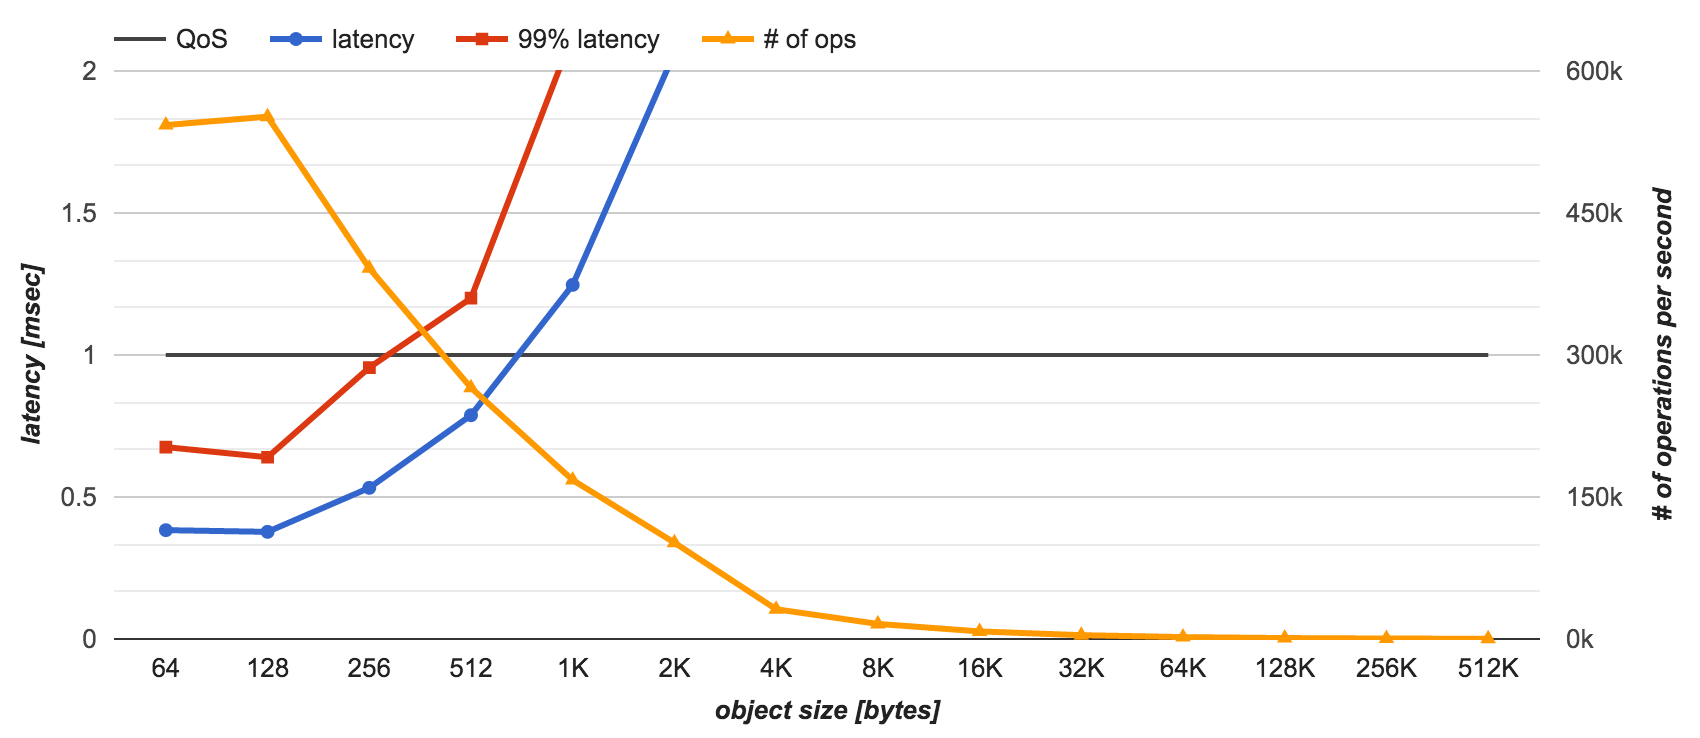
\includegraphics[width=\textwidth]{./res2/m_object_size_latency.png}
    \caption{CPU Utilization with Multiple Instances}
    \label{fig:m_object_size_latency}
\end{figure}

Figure \ref{fig:m_object_size_latency} plots the relationship between object size, latency and throughput. As object size increases the number of operations decreases while the 99th percentile latency increases. This is an expected result as larger object sizes will incur increased latency. Similar results are reported by \cite{lim2013thin}. Interestingly, with object sizes of 128 bytes we achieve the highest throughput with the smallest tail latency, however, this result is overshadowed by the overall trend of object size.

The QoS requirements are satisfied with object sizes between 64 and 256 bytes. With objects larger, we are no longer able to provide the required QoS.


\subsection{CPU vs Object Size}

\begin{figure}[h]
    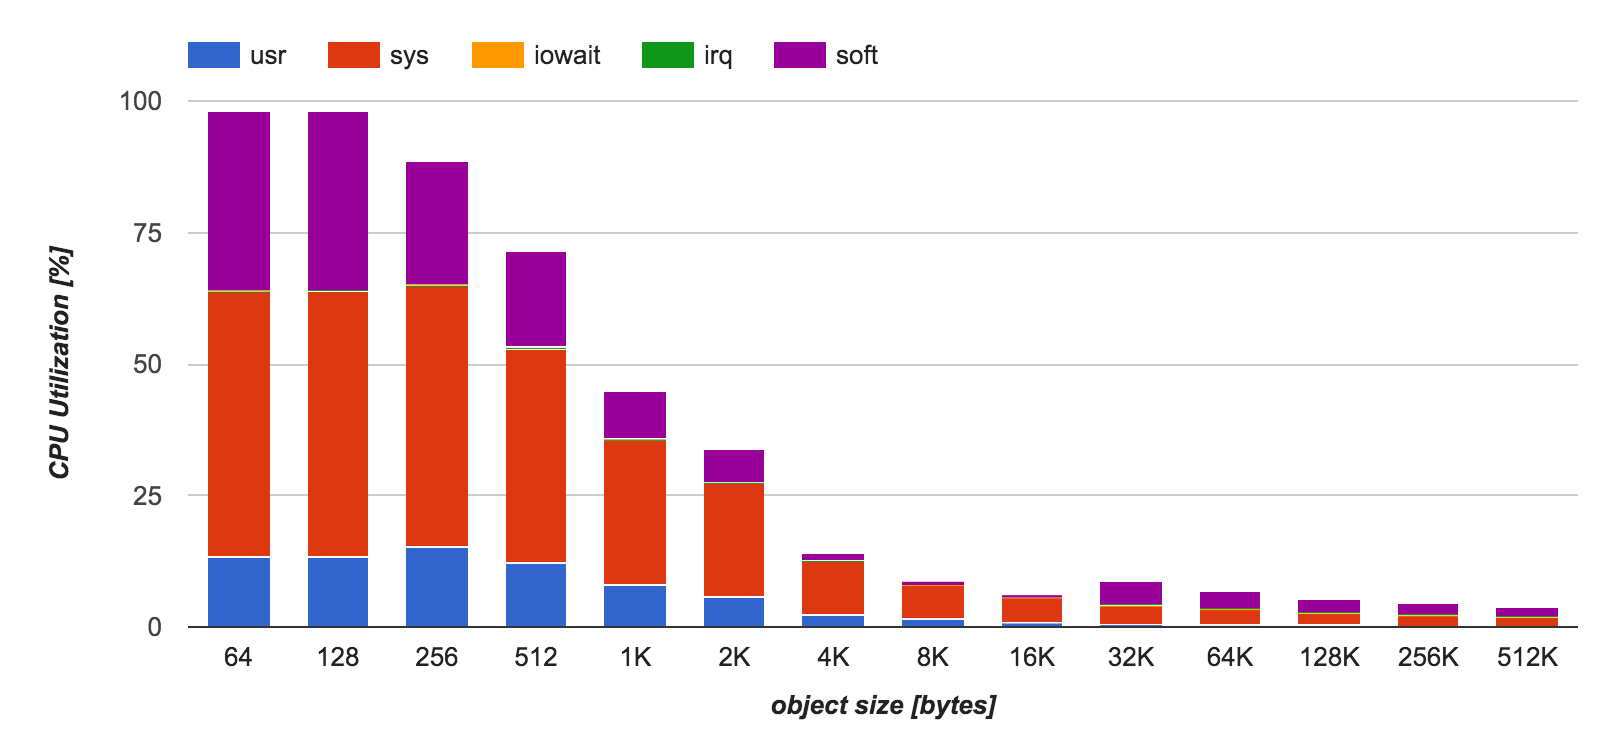
\includegraphics[width=\textwidth]{./res2/m_object_size_cpu.png}
    \caption{CPU Utilization with Multiple Instances}
    \label{fig:m_object_size_cpu}
\end{figure}

Figure \ref{fig:m_object_size_cpu} plots the CPU utilization against each object size. Overall, we achieve high CPU utilization with only objects of size 64 and 128 bytes. As the object size decreases, the total CPU utilization decreases too. The individual category breakdown remains the same with majority of CPU used by the kernel followed by software interrupts.

As object size increases, the network performance begins to dominate over the performance of the cache and/or the host CPU. Smaller objects, on the other hand, are processing constrained \cite{lim2013thin}.

\subsection{Object Size Conclusion}
In this section, we have explored Memcached scalability with respect to object size. Our benchmarks show that Memcached scales well up to objects of size 256 bytes. Larger objects result in significant penalties in terms of throughput and tail latency. Reducing the load on our cache server, we would be able to obtain better scalability in terms of object size at the expense of throughput. Additionally, we have argued that large objects are predominantly network dependent. A faster NIC with corresponding switch interconnect would likely provide better scalability. In an analysis of Facebook Memcached workloads, a dominant portion of all object sizes fall below 270 bytes \cite{atikoglu2012workload}. It is further argued that ``small values dominate all workloads, not just in count, but especially in overall weight.'' \cite{atikoglu2012workload} We can conclude that Memcached does not scale well for objects larger than 512 bytes. In practice, application design and architecture decisions can be made to either optimize Memcached for large object size performance and/or use many smaller objects with client side re-assembly.


% ---------------------------------------------------------------
\section{Key Distribution}
\label{sec:memcached_zipf}
In this section, we investigate the effect of a skewed key distribution on the cache performance. In practice, ``most web objects follows a zipf-like distribution, although the exact slope may vary'' \cite{lim2013thin}.

We consider a Zipf distribution defined by the following frequency function

$f(k; s, N) = \frac{1 / k^s}{\sum_{n=1}^{N} (1 / n^s)}$

where $k$ represents a given key, $s$ represents an exponent describing the distribution (also called the zipf factor) and $N$ is the total number of keys. Figure \ref{fig:zipf} plots the cumulative density function produced for a 10 million key range with varying values of $s$.

\begin{figure}[h]
    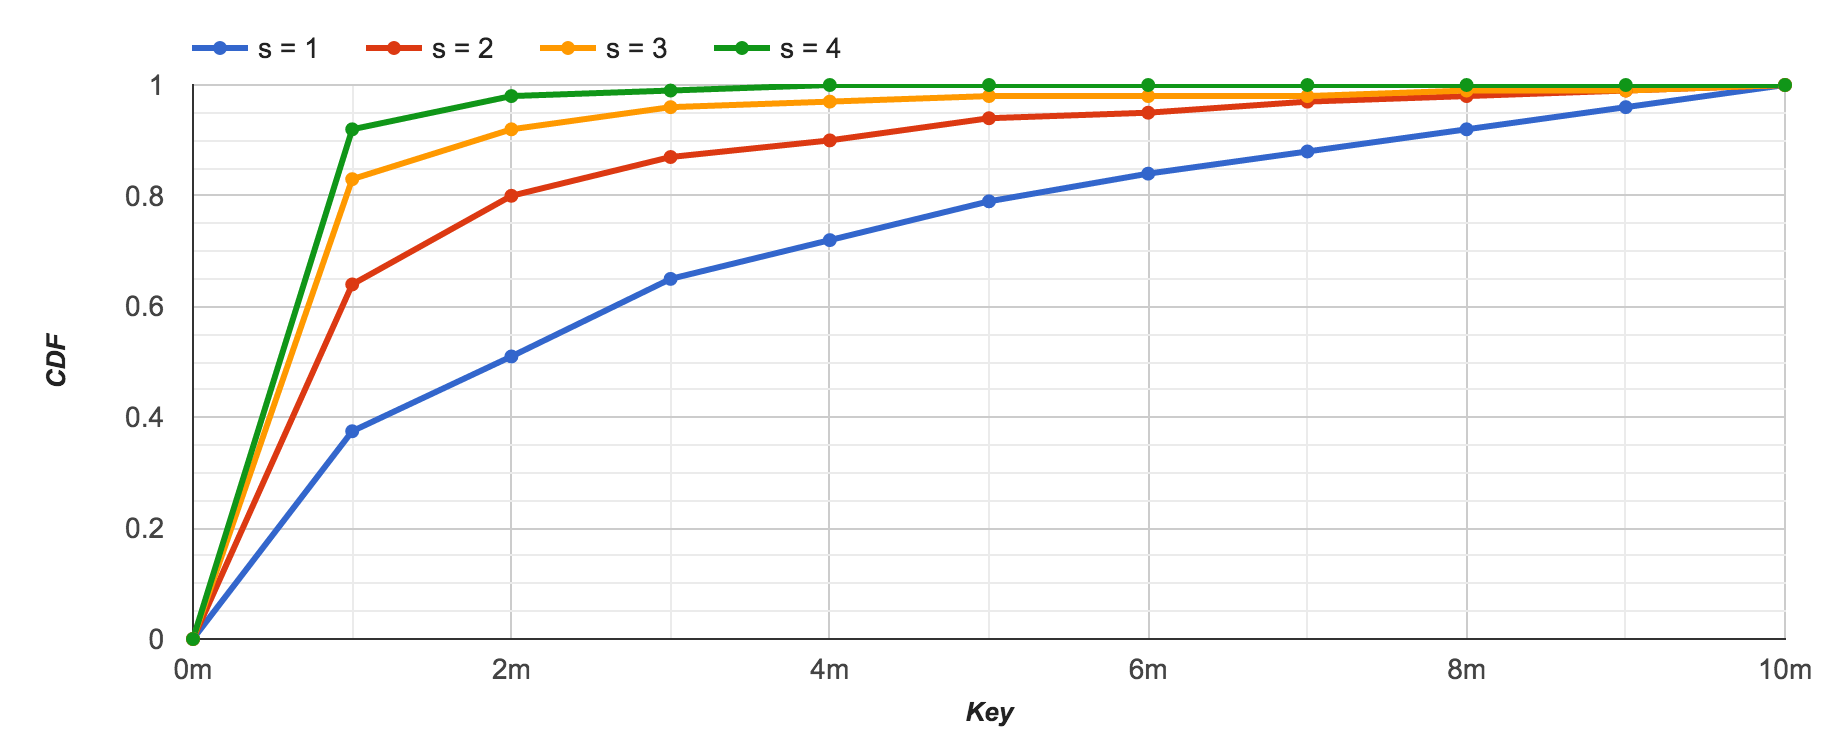
\includegraphics[width=\textwidth]{./res2/zipf.png}
    \caption{Zipf Cumulative Density Function with different values of s}
    \label{fig:zipf}
\end{figure}

In order to generate a zipf-like distribution with Memtier, a fork of memtier with modified implementation is used as the official implementation does not support the zipf distribution.

\subsection{Latency \& Throughput}
\begin{figure}[h]
    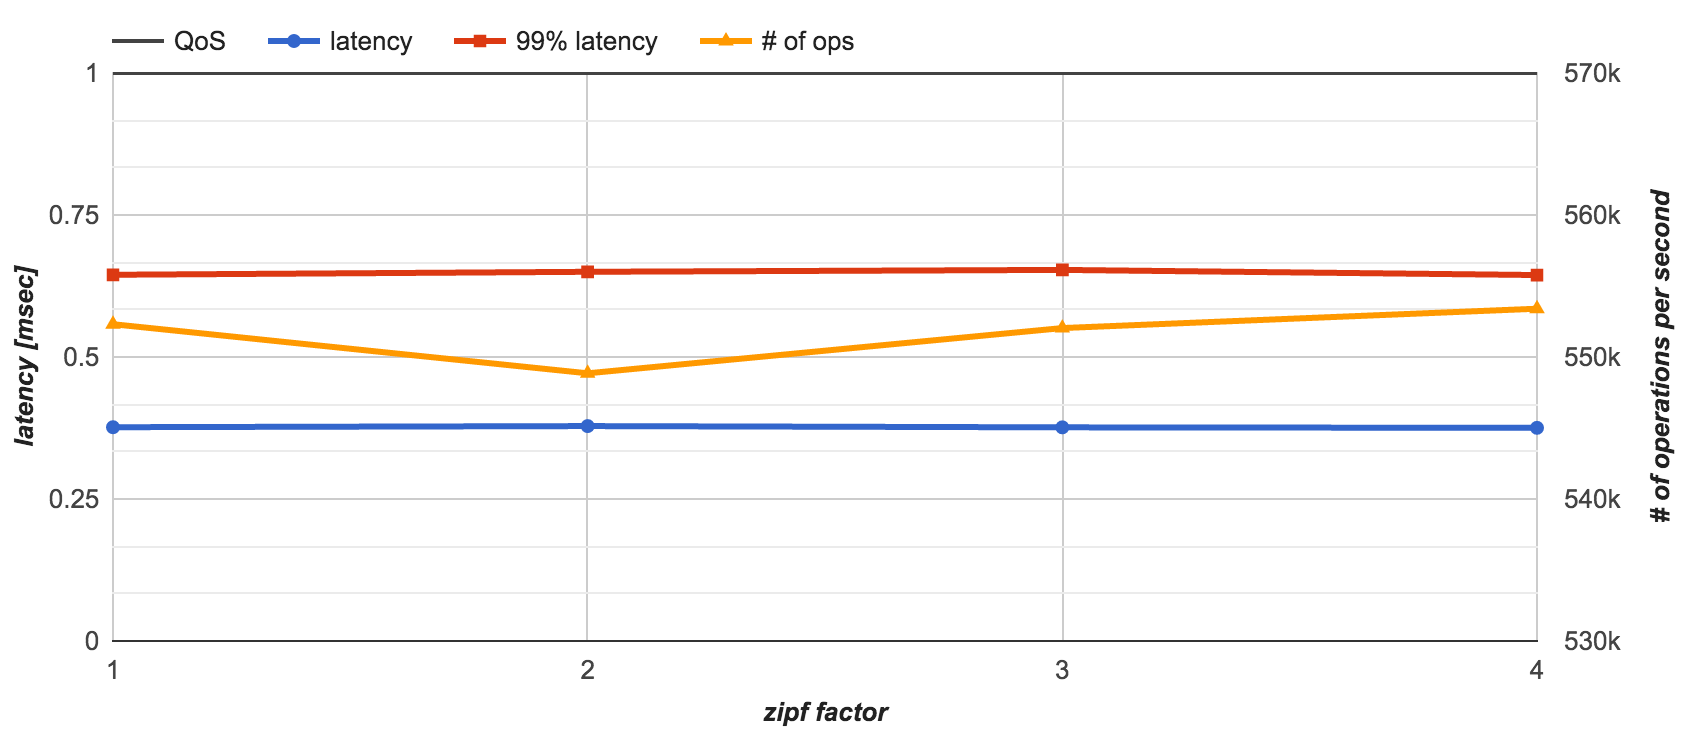
\includegraphics[width=\textwidth]{./res2/m_zipf.png}
    \caption{Memcached with Zipf-like key distribution}
    \label{fig:m_zipf}
\end{figure}

Figure \ref{fig:m_zipf} plots the relationship between latency, operations per second and the zipf factor. The higher the zipf factor, the more heavily skewed the distribution is. Overall, mean and 99th percentile latency remain nearly constant. Operations per second drop slightly at zipf factor of 2, however, on the relative scale of the operations per second it is rather insignificant.

The CPU utilization with a Zipf distribution remains the same as in Figure \ref{fig:m_threads_irq_cpu}.

We find that there is no significant difference in overall performance of Memcached nor in CPU utilization with a zipf-like distribution. However, we also find that a Zipf-like key distribution increases throughput as opposed to a uniformly random distribution. We obtain an increase of 10k requests per second as opposed to results obtained after IRQ pinning.

